\documentclass[11pt]{article}

\usepackage{graphicx}			% Use this package to include images
\usepackage{amsmath}			% A library of many standard math expressions
\usepackage{amsfonts}
\usepackage[margin=1in]{geometry}% Sets 1in margins.
\usepackage{fancyhdr}			% Creates headers and footers
\usepackage{enumerate}          %These two package give custom labels to a list
\usepackage[shortlabels]{enumitem}
\usepackage{braket}
\usepackage{physics}
\usepackage{pgfplots}
\usepackage{tikz}
\usepackage{xcolor}
\usepackage{mathtools}
\usepackage{url}
\usepackage{listings}
\usepackage{geometry}

%% LISTINGS CONFIG %%

\definecolor{purple2}{RGB}{153,0,153} % there's actually no standard purple
\definecolor{green2}{RGB}{0,153,0} % a darker green

\lstset{
  language=Python,                   % the language
  basicstyle=\normalsize\ttfamily,   % size of the fonts for the code
  frame = single,
  % Color settings to match IDLE style
  keywordstyle=\color{orange},       % core keywords
  keywordstyle={[2]\color{purple2}}, % built-ins
  stringstyle=\color{green2},%
  showstringspaces=false,
  commentstyle=\color{red},%
  upquote=true,                      % requires textcomp
  numbers=left,
  breaklines=true,
}


\title{\textbf{ECE469 Homework 2}}
\author{Chase A. Lotito}
\date{\today}

\begin{document} %The writing for your homework should all come after this.

\maketitle


\section*{Question 1}

\textbf{Solution.}

% code from q1.py
\begin{center}
  q1.py
\end{center}
\begin{lstlisting}
###########################
# Chase Lotito - SIUC F24 #
# ECE469 - Intro to ML    #
# HW2 - Question 1        #
###########################

# IMPORT LIBRARIES
import numpy as np
import pandas as pd
import matplotlib.pyplot as plt
from sklearn.preprocessing import PolynomialFeatures
from sklearn.model_selection import cross_val_score, train_test_split, KFold
from sklearn.linear_model import LinearRegression
from sklearn.linear_model import Ridge
from sklearn.metrics import mean_squared_error

# Read in provided csv data to pandas dataframe
RAW_DATA_PATH = 'C:/Users/cloti/OneDrive/Desktop/CODE/datasets/datasetHW2P1.csv'
data = pd.read_csv(RAW_DATA_PATH)

test_size = 0.2


# (A) SPLIT DATASET TO CREATE TWO SUB DATASETS FOR TRAINING AND TESTING
x = data['x'].values
y = data['y'].values

x = x.reshape(-1, 1)

x_train, x_test, y_train, y_test = train_test_split(x, y, test_size=test_size, random_state=42)




# (B) USE POLYNOMIAL REGRESSION TO FIT 5 POLYNOMIAL MODELS (DEG. 1 - DEG. 5)
deg = [1, 2, 3, 4, 5]
mse_train_arr = []
mse_test_arr = []

for i in deg:
    # transform input features into polynomial features
    poly = PolynomialFeatures(degree=i)    # initialize polynomial
    x_train_poly = poly.fit_transform(x_train)
    x_test_poly = poly.transform(x_test)

    # fit model
    poly_regressor = LinearRegression()
    poly_regressor.fit(x_train_poly, y_train)

    # test
    y_train_predicted = poly_regressor.predict(x_train_poly)
    y_test_predicted = poly_regressor.predict(x_test_poly)

    # calc mse
    mse_train = mean_squared_error(y_train, y_train_predicted)
    mse_test = mean_squared_error(y_test, y_test_predicted)

    # add mse's to arrays for later plotting
    mse_train_arr.append(mse_train)
    mse_test_arr.append(mse_test)

    # print mse for training and testing
    print(f"Degree: {i}")
    print(f"MSE Training: {mse_train}")
    print(f"MSE Testing: {mse_test}")

# plotting mse for training and testing against model complexity
plt.plot(deg, mse_train_arr, label='Training')
plt.plot(deg, mse_test_arr, label='Testing')
plt.xlabel('Model Complexity (Degree)')
plt.ylabel('Mean Square Error')
plt.title('Model Error v. Model Complexity')
plt.legend()
#plt.show()
#plt.close()




# (C) USE 10-FOLD CROSS-VALIDATION TO FIND THE MODEL WHICH OPTIMALLY FITS GIVEN DATASET.
#     PLOT THE TRAINING, CROSS-VALIDATION, AND TESTING ERRORS AGAINST MODEL COMPLEXITY.

# parameters
k = 10                 # for 10-fold cross-validation
best_degree = 1        # track best degree
max_degree = 5
best_mse = float('inf')
mse_per_degree = []

# perform k-fold cross-validation for each polynomial degree
for degree in range(1, max_degree + 1):
    kf = KFold(n_splits=k, shuffle=True, random_state=42)
    mse_fold_values = []
    k_iter = 1

    # initialize a plot for regression fit
    all_y_pred = np.zeros(x.shape)

    # Loop through each fold
    for train_index, test_index in kf.split(x):
        x_train, x_test = x[train_index], x[test_index]
        y_train, y_test = y[train_index], y[test_index] 

        # transform original x data into polynomial features for current degree
        poly = PolynomialFeatures(degree=degree)    # here degree is the parent loop iterator
        x_train_poly = poly.fit_transform(x_train)
        x_test_poly = poly.transform(x_test)

        # intialize and fit linear regression on polynomial space input features
        poly_regressor = LinearRegression()
        poly_regressor.fit(x_train_poly, y_train)         # <-- TRAINING MODEL HERE

        # predict using trained model
        y_test_pred = poly_regressor.predict(x_test_poly)

        # calc mse for test set
        mse_test = mean_squared_error(y_test, y_test_pred)
        mse_fold_values.append(mse_test)

    # calculuate avg mse for all folds for current deg
    avg_mse = np.mean(mse_fold_values)
    mse_per_degree.append(avg_mse)

    # check if current deg has lowest avg mse
    if avg_mse < best_mse:
        best_mse = avg_mse
        best_degree = degree
    

    # Generate new plot for degree
    plt.figure(figsize=(12,8))
    plt.scatter(x,y,s=10,color='blue', label='Original Data', alpha=0.6)

    # plot polynomial fit for degree
    sorted_x = np.sort(x, axis=0)
    sorted_x_poly = poly.transform(sorted_x)
    plt.plot(sorted_x, poly_regressor.predict(sorted_x_poly), color='red', label=f"Degree {degree}", alpha = 0.7)

    # finalize plot for degree
    plt.title(f"Polynomial Regression (Degree {degree})")
    plt.xlabel('x')
    plt.ylabel('y')
    plt.legend(loc='best')
    plt.grid(True)
    plt.savefig(f"poly_reg_deg{degree}_fold{k_iter}.png", dpi=300)
    plt.close()

# print best degree and mse
print(f"Best Polynomial Degree: {best_degree}")

# plot the mse v. polynomial degree
plt.figure(figsize=(10,6))
plt.plot([1,2,3,4,5], mse_per_degree, marker='o', color='b', label='Cross-Validation MSE', alpha=0.75)
plt.plot(deg, mse_train_arr, label='Training MSE', marker='+', alpha=0.75)
plt.plot(deg, mse_test_arr, label='Testing MSE', marker='x', alpha=0.75)
plt.title("MSE vs Model Complexity")
plt.xlabel('Polynomial Degree')
plt.ylabel('Mean Squared Error (MSE)')
plt.xticks(range(1, max_degree + 1))
plt.legend()
plt.grid(True)
plt.savefig('plots\\mse_vs_complexity.png', dpi=300)
plt.close()




# (D) CONSIDER A 4-DEGREE POLYNOMIAL AS YOUR MODEL.
#     USE RIDGE REGRESSION AND FIND BEST HYPERPARAMETER
#     LAMBDA VIA 10-F0LD CROSS-VALIDATION. PLOT THE CROSS
#     VALIDATION ERROR VERSUS LN(LAMBDA).

# remember we have x as input features and y as output features

# parameters
degree = 4                         # polynomial degree
lambdas = np.logspace(-4, 2, 100)  # lambdas for ridge
kf = KFold(n_splits=10, shuffle=True, random_state=1)

# map input features into its polynomial space
poly = PolynomialFeatures(degree=degree)
x_poly = poly.fit_transform(x)

# store cross-validation results
mse_values = []

# perform cross-validation for each lambda
for alpha in lambdas:
    ridge = Ridge(alpha=alpha)

    # calc mse using cross_val_score
    mse = -cross_val_score(ridge, x_poly, y, cv=kf, scoring='neg_mean_squared_error').mean()
    mse_values.append(mse)

# find lambda with best minimum mse
best_lambda = lambdas[np.argmin(mse_values)]
print(f"Best lambda (w/ minimum MSE): {best_lambda}")

# fit model with best lambda
ridge_best = Ridge(alpha=best_lambda)
ridge_best.fit(x_poly, y)

# generate testing x values
x_fit = np.linspace(x.min(), x.max(), 1000).reshape(-1,1)
x_poly_fit = poly.transform(x_fit)   # send x_fit to polynomial space
y_fit = ridge_best.predict(x_poly_fit)

# plot mse vs. ln(lambda)
plt.figure(figsize=(8,6))
plt.plot(np.log(lambdas), mse_values, label='MSE')
plt.xlabel('$\\log_e (\\lambda)$')
plt.ylabel('Cross-Validated MSE')
plt.title('Cross-Validated MSE v. $\\log_e (\\lambda)$')
plt.grid(True)
plt.legend()
plt.savefig('crossvalmse_vs_loglambda.png', dpi=300)
plt.close()
\end{lstlisting}


\begin{figure}[h!]
  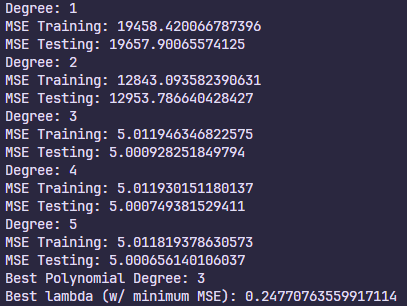
\includegraphics[width=0.5\textwidth]{../outputs/q1.png}
  \centering
  \caption{q1.py Terminal Output}
  \label{fig:q1out}
\end{figure}

\begin{figure}[h!]
  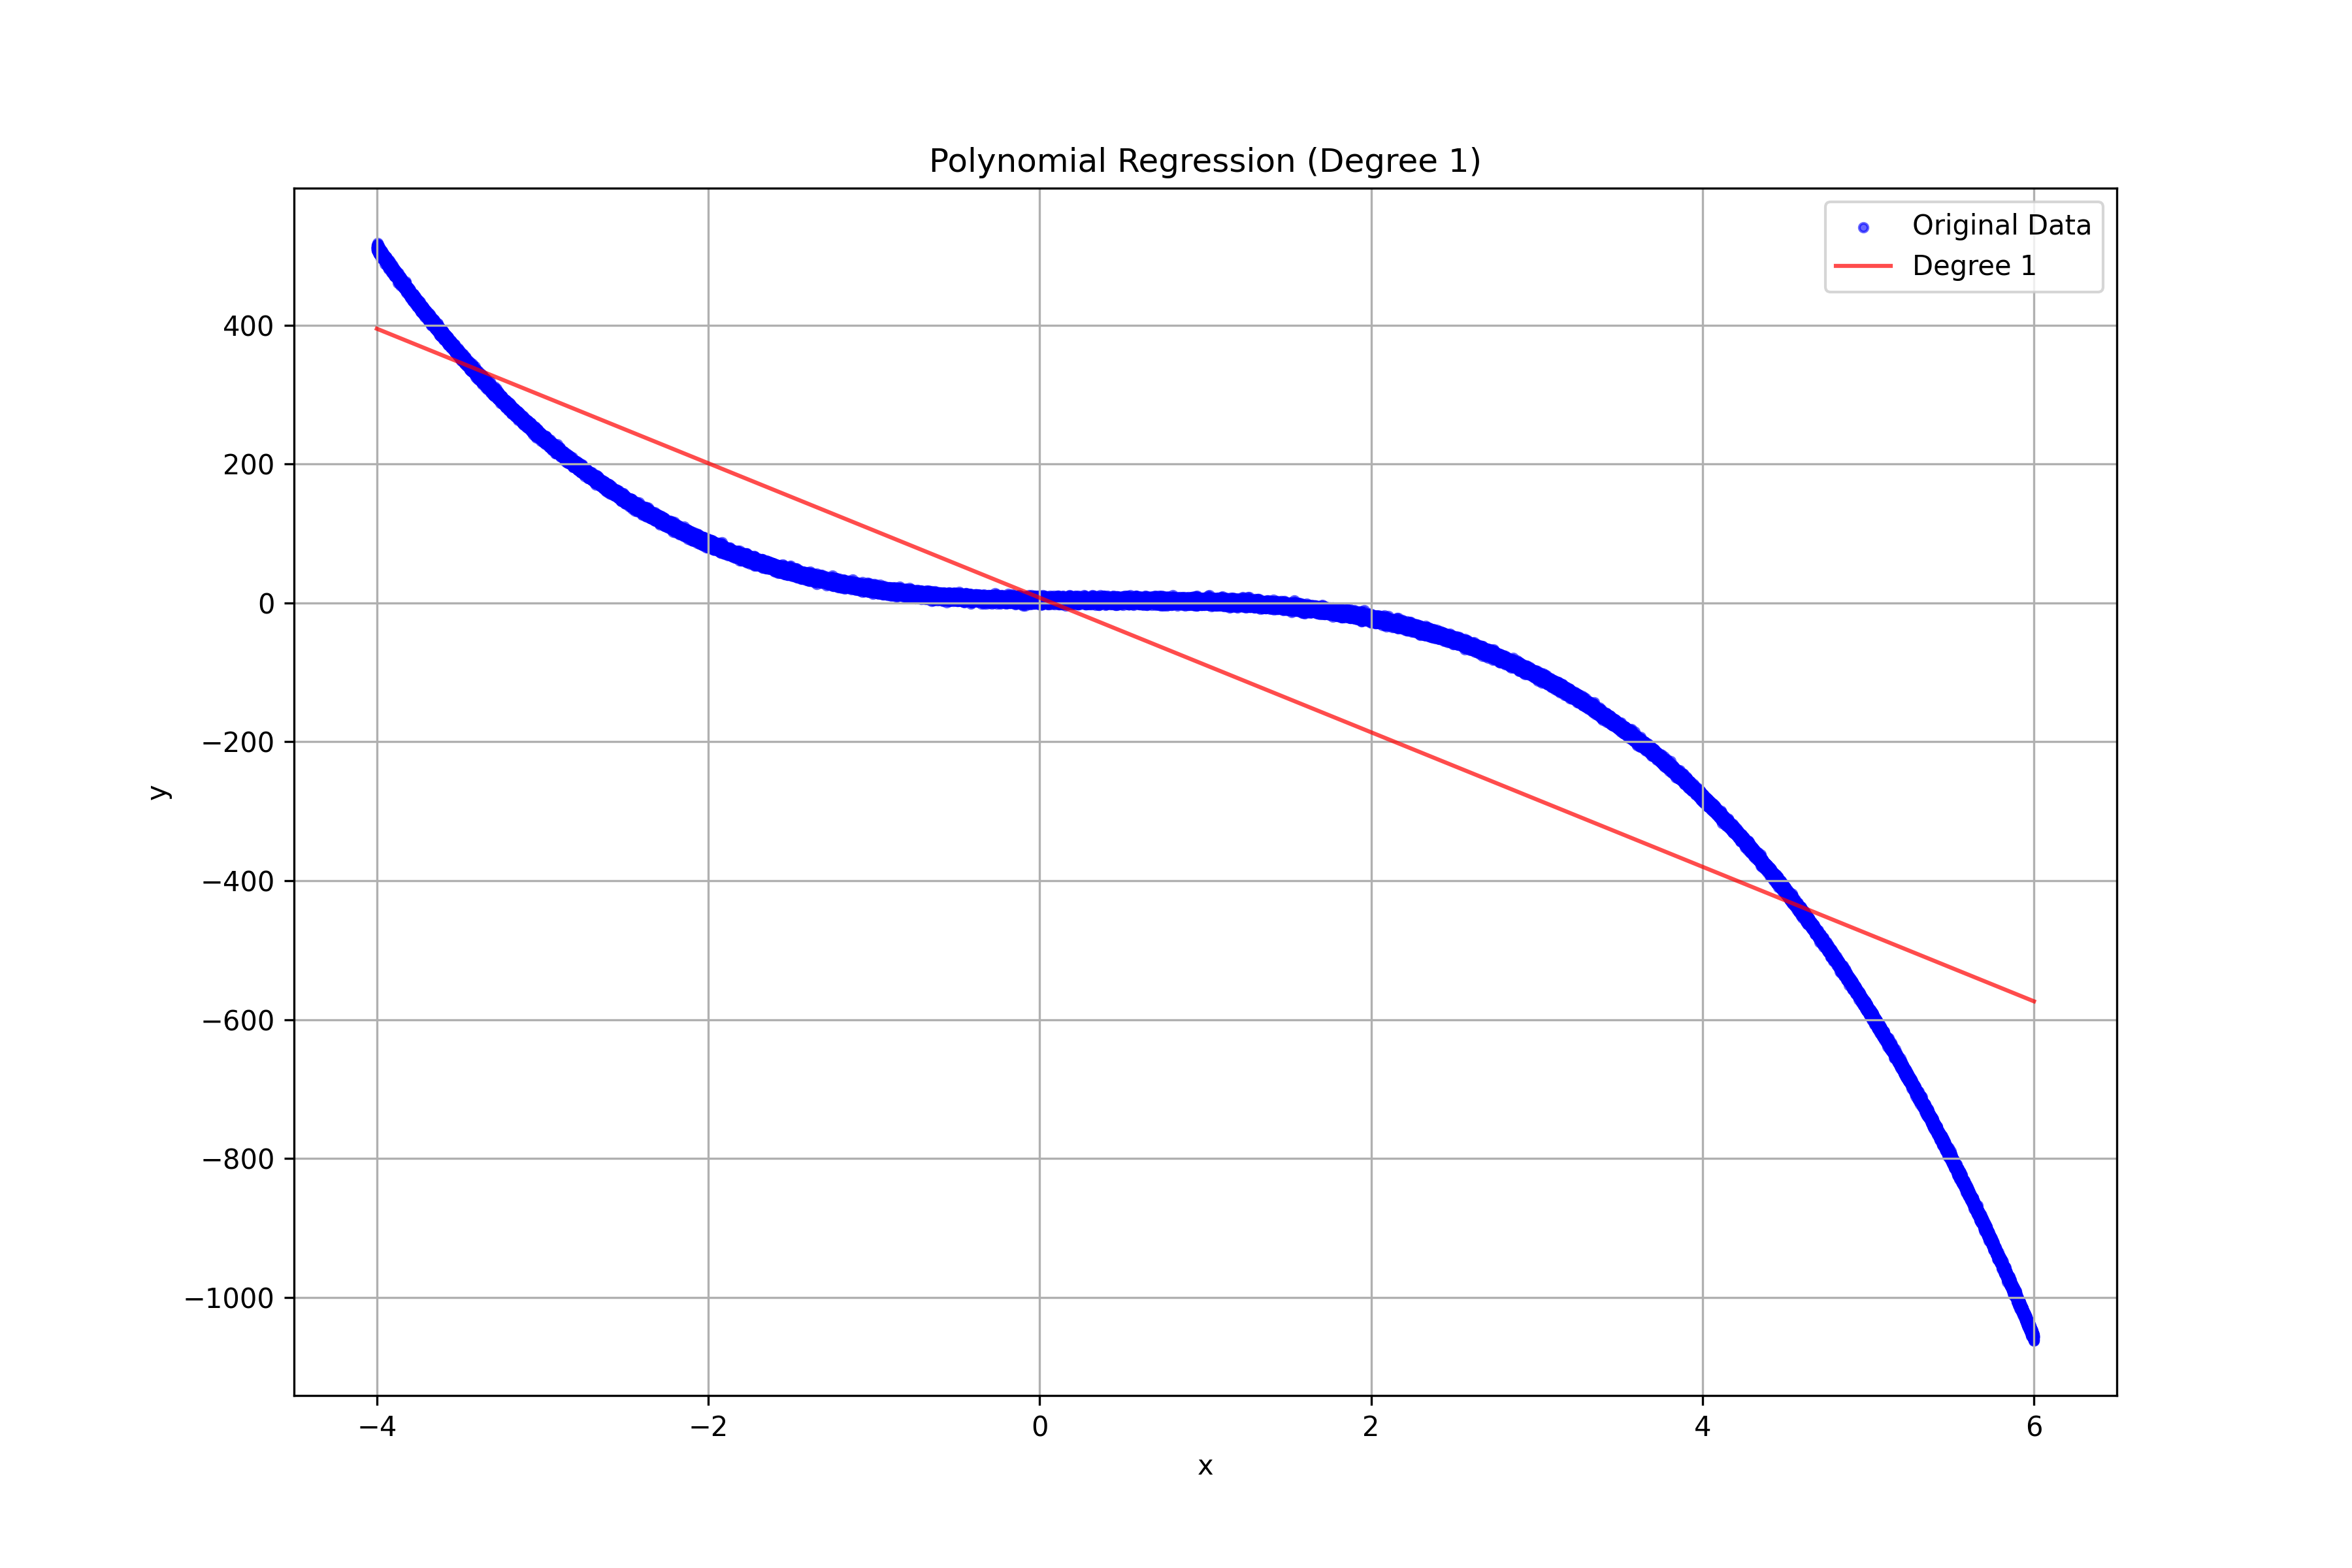
\includegraphics[width=\textwidth]{../plots/poly_reg_deg1_fold1.png}
  \centering
  \caption{Polynomial Model Degree 1}
\end{figure}

\begin{figure}[h!]
  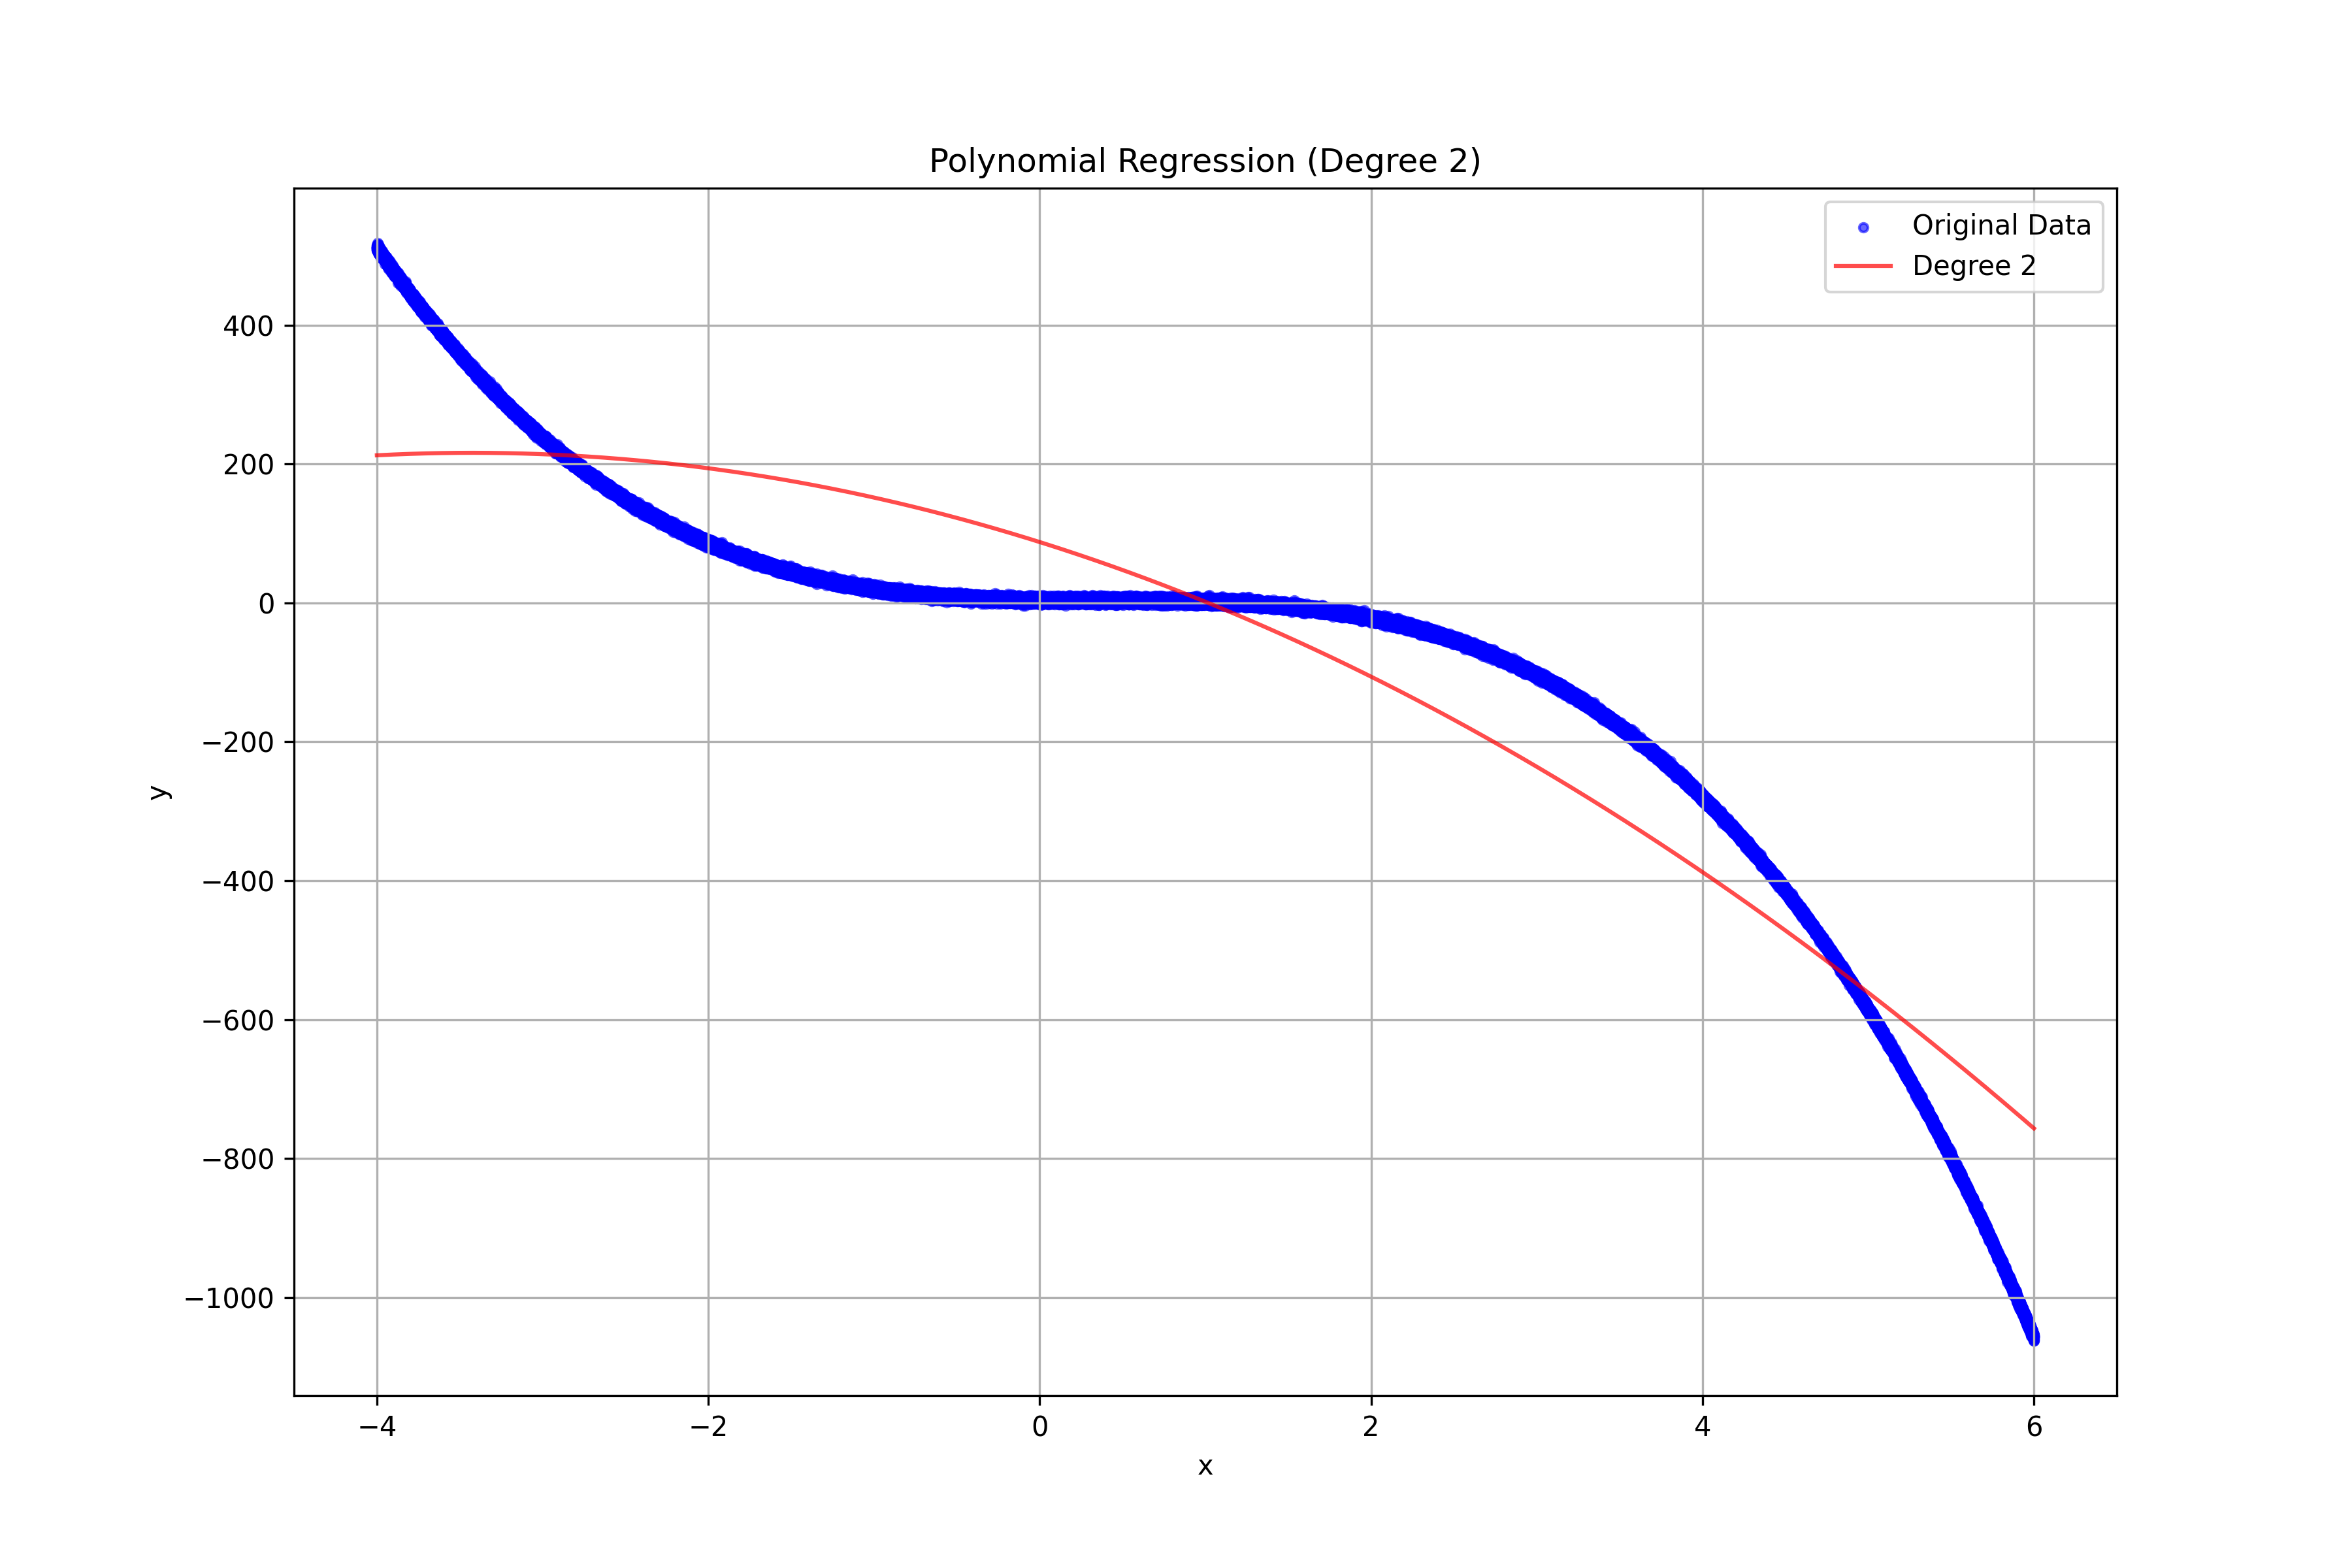
\includegraphics[width=\textwidth]{../plots/poly_reg_deg2_fold1.png}
  \centering
  \caption{Polynomial Model Degree 2}
\end{figure}

\begin{figure}[h!]
  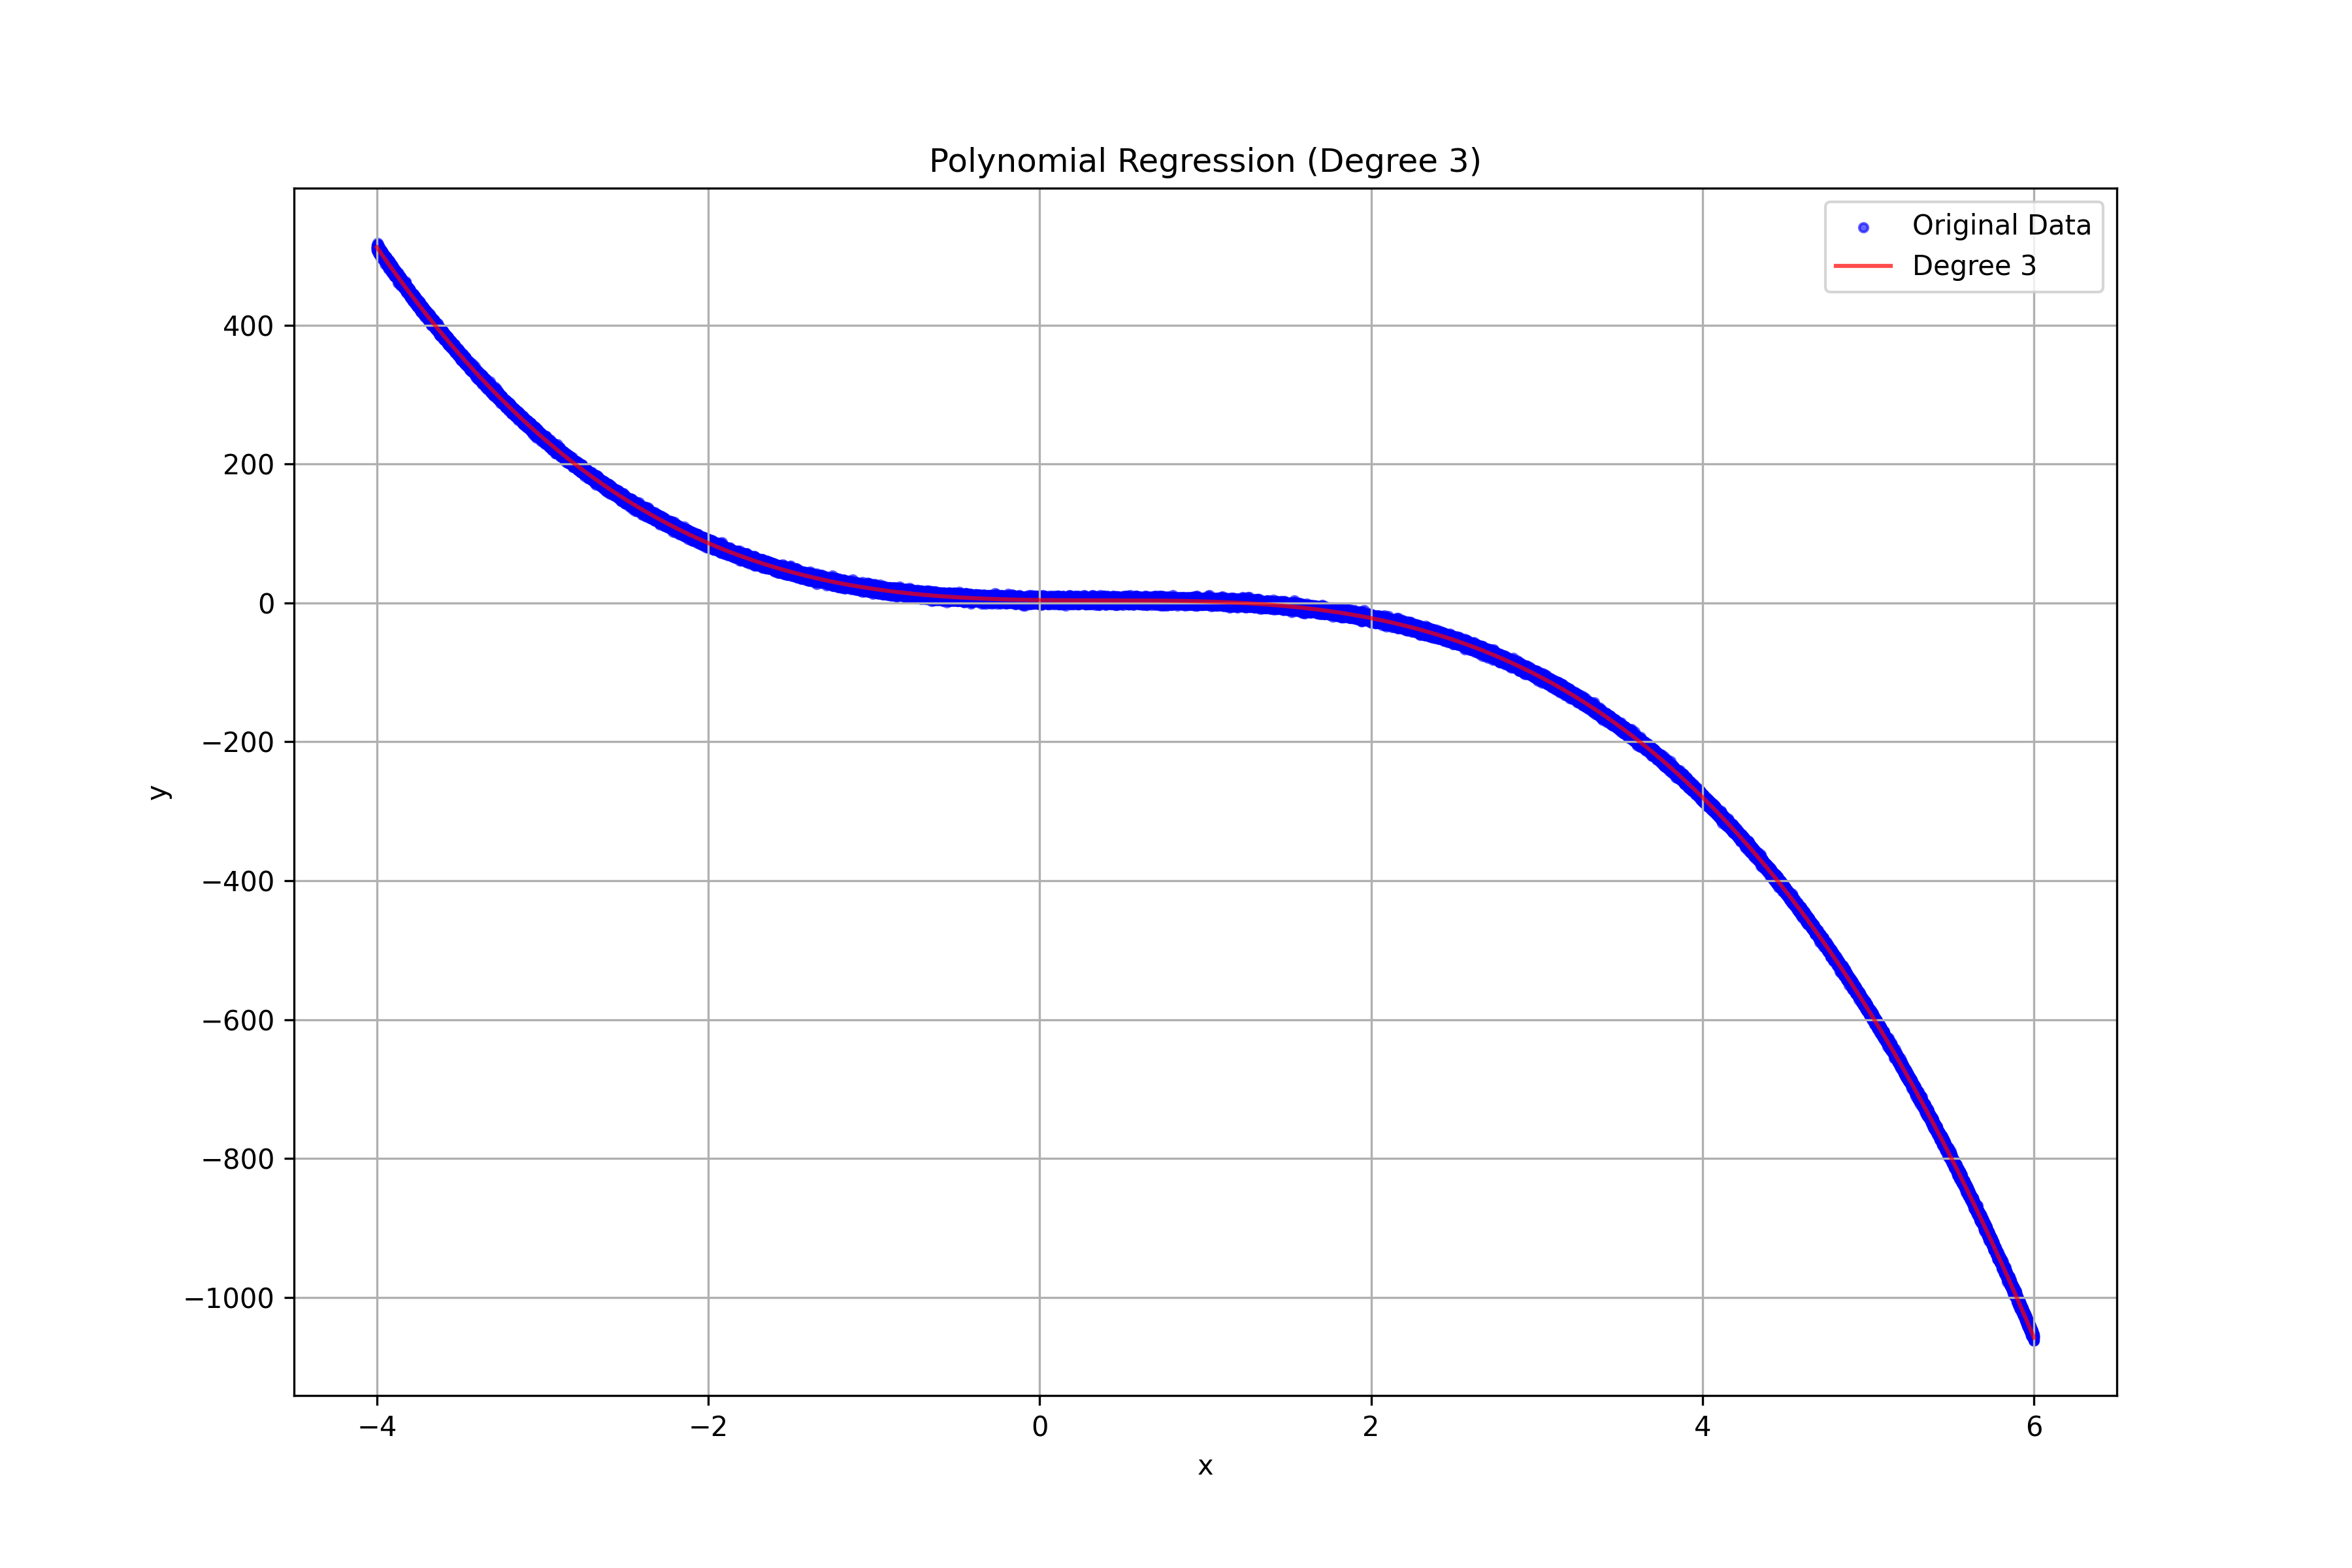
\includegraphics[width=\textwidth]{../plots/poly_reg_deg3_fold1.png}
  \centering
  \caption{Polynomial Model Degree 3}
\end{figure}

\begin{figure}[h!]
  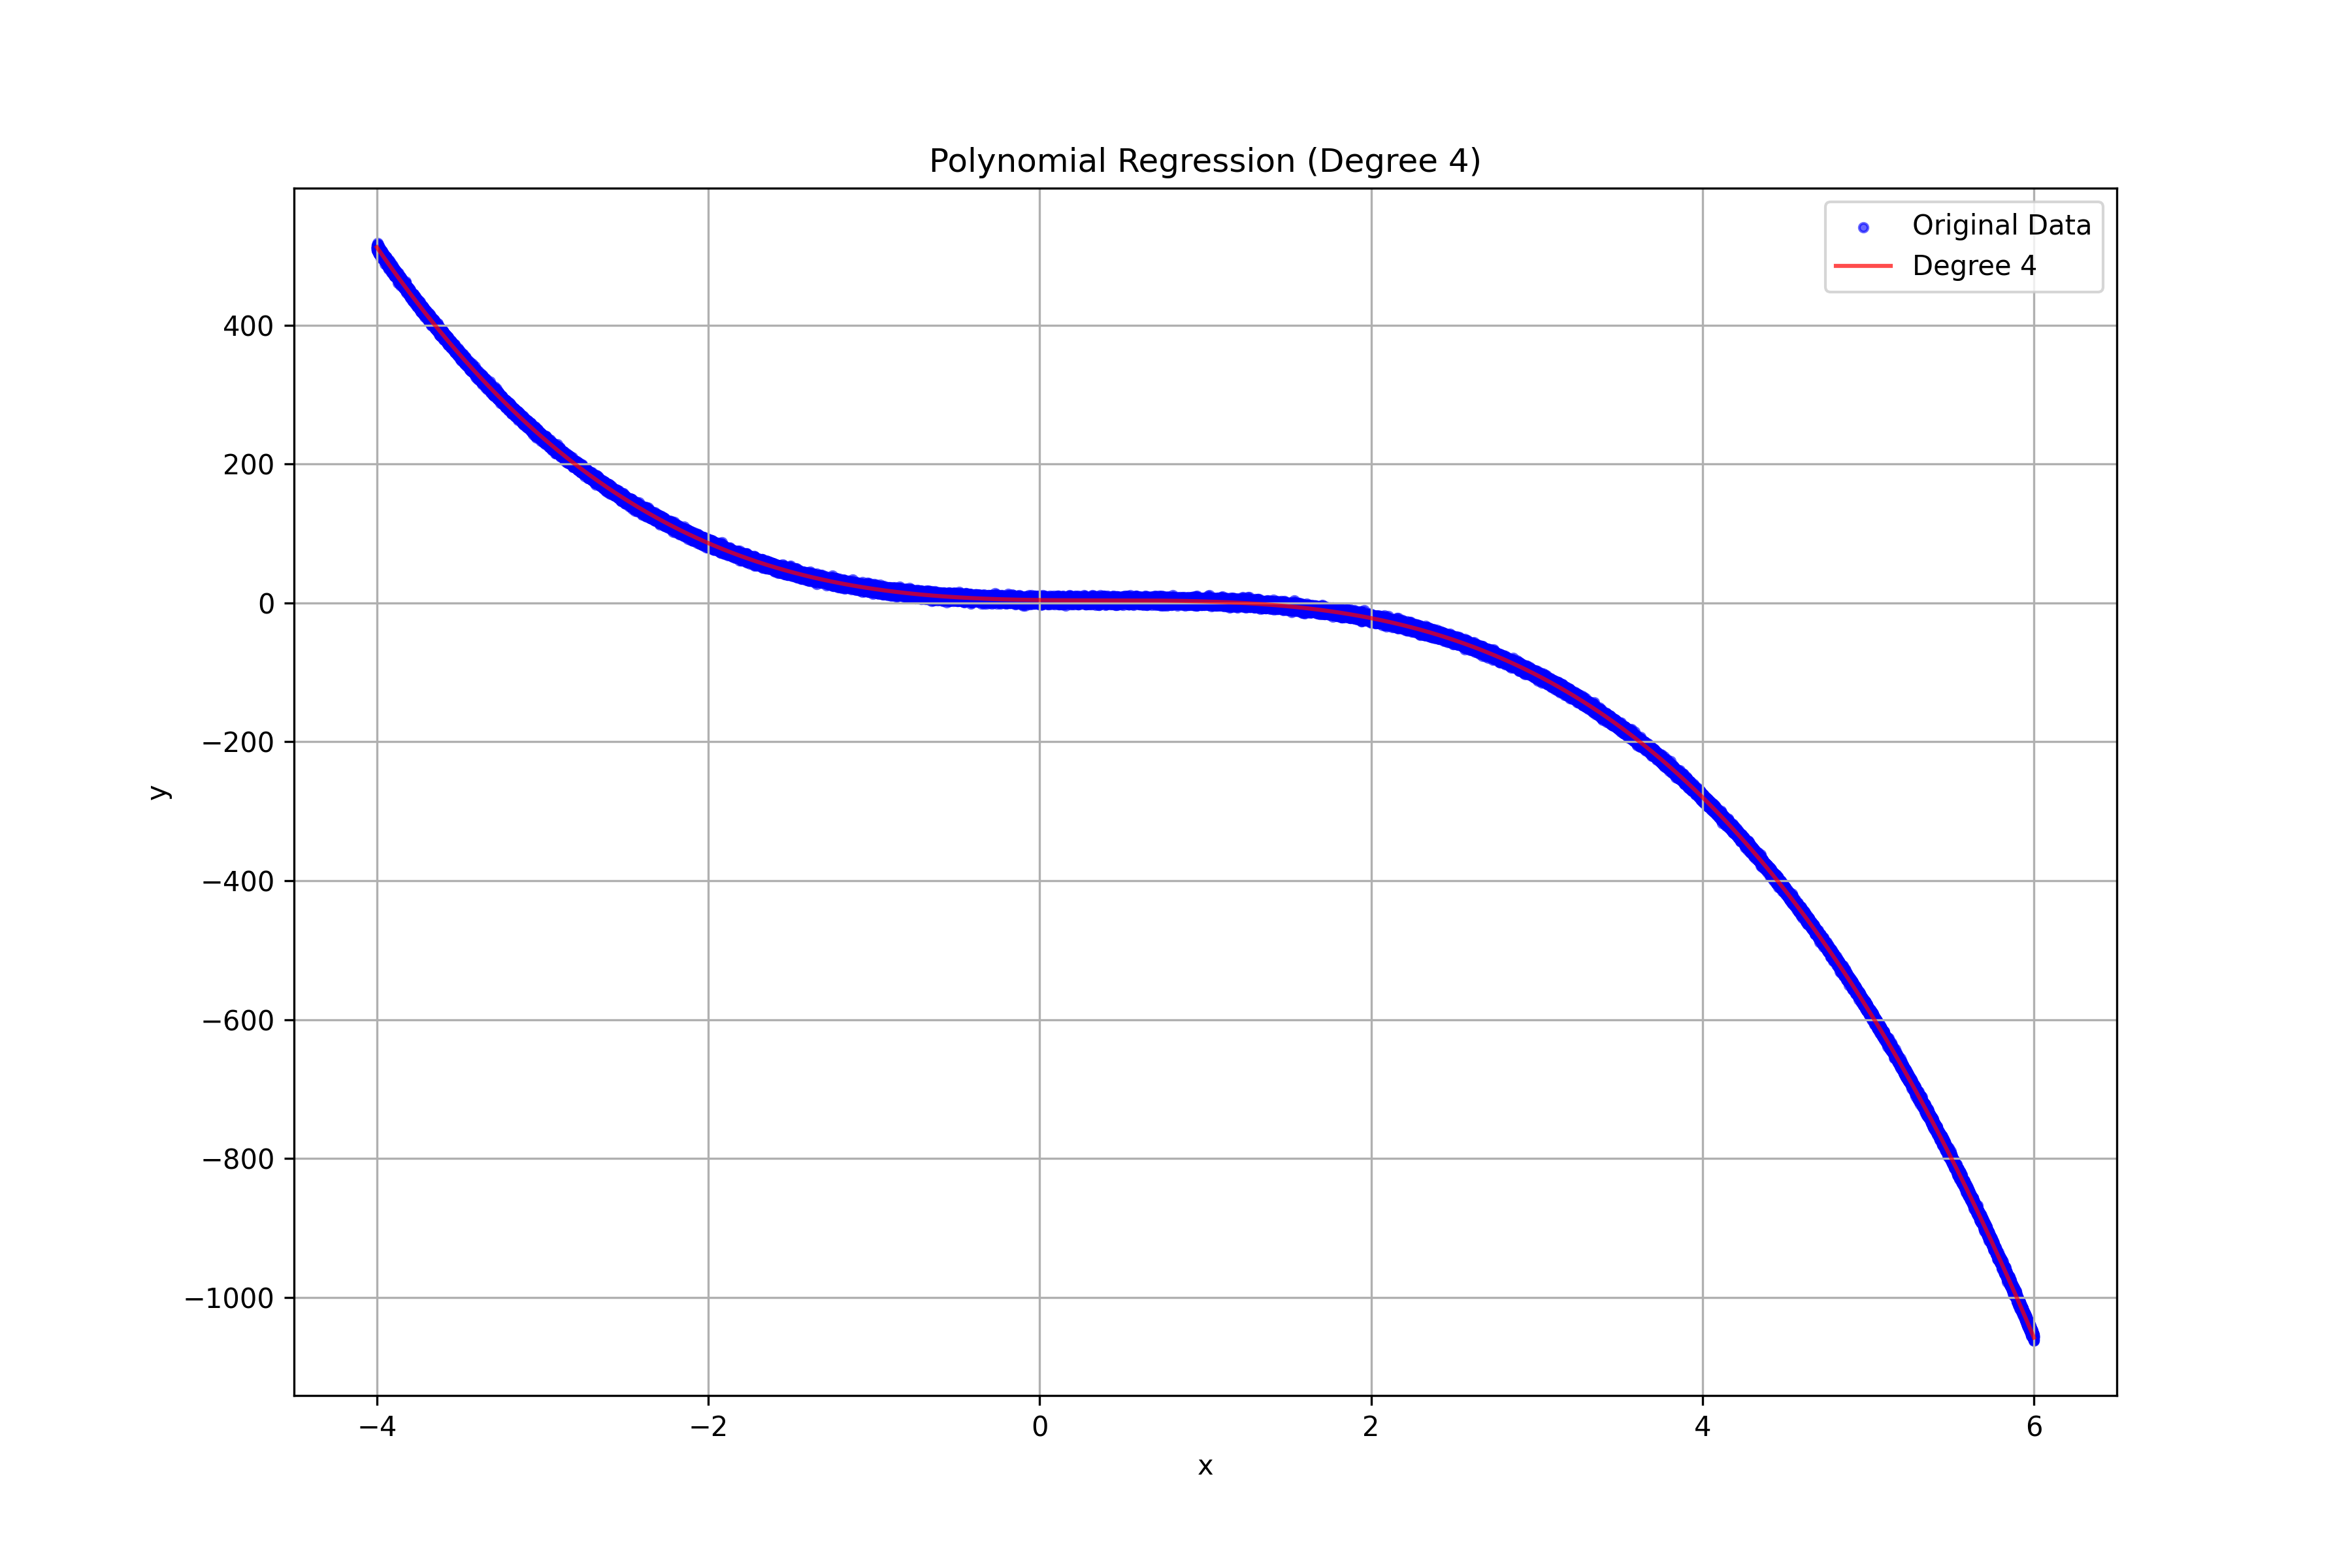
\includegraphics[width=\textwidth]{../plots/poly_reg_deg4_fold1.png}
  \centering
  \caption{Polynomial Model Degree 4}
\end{figure}

\begin{figure}[h!]
  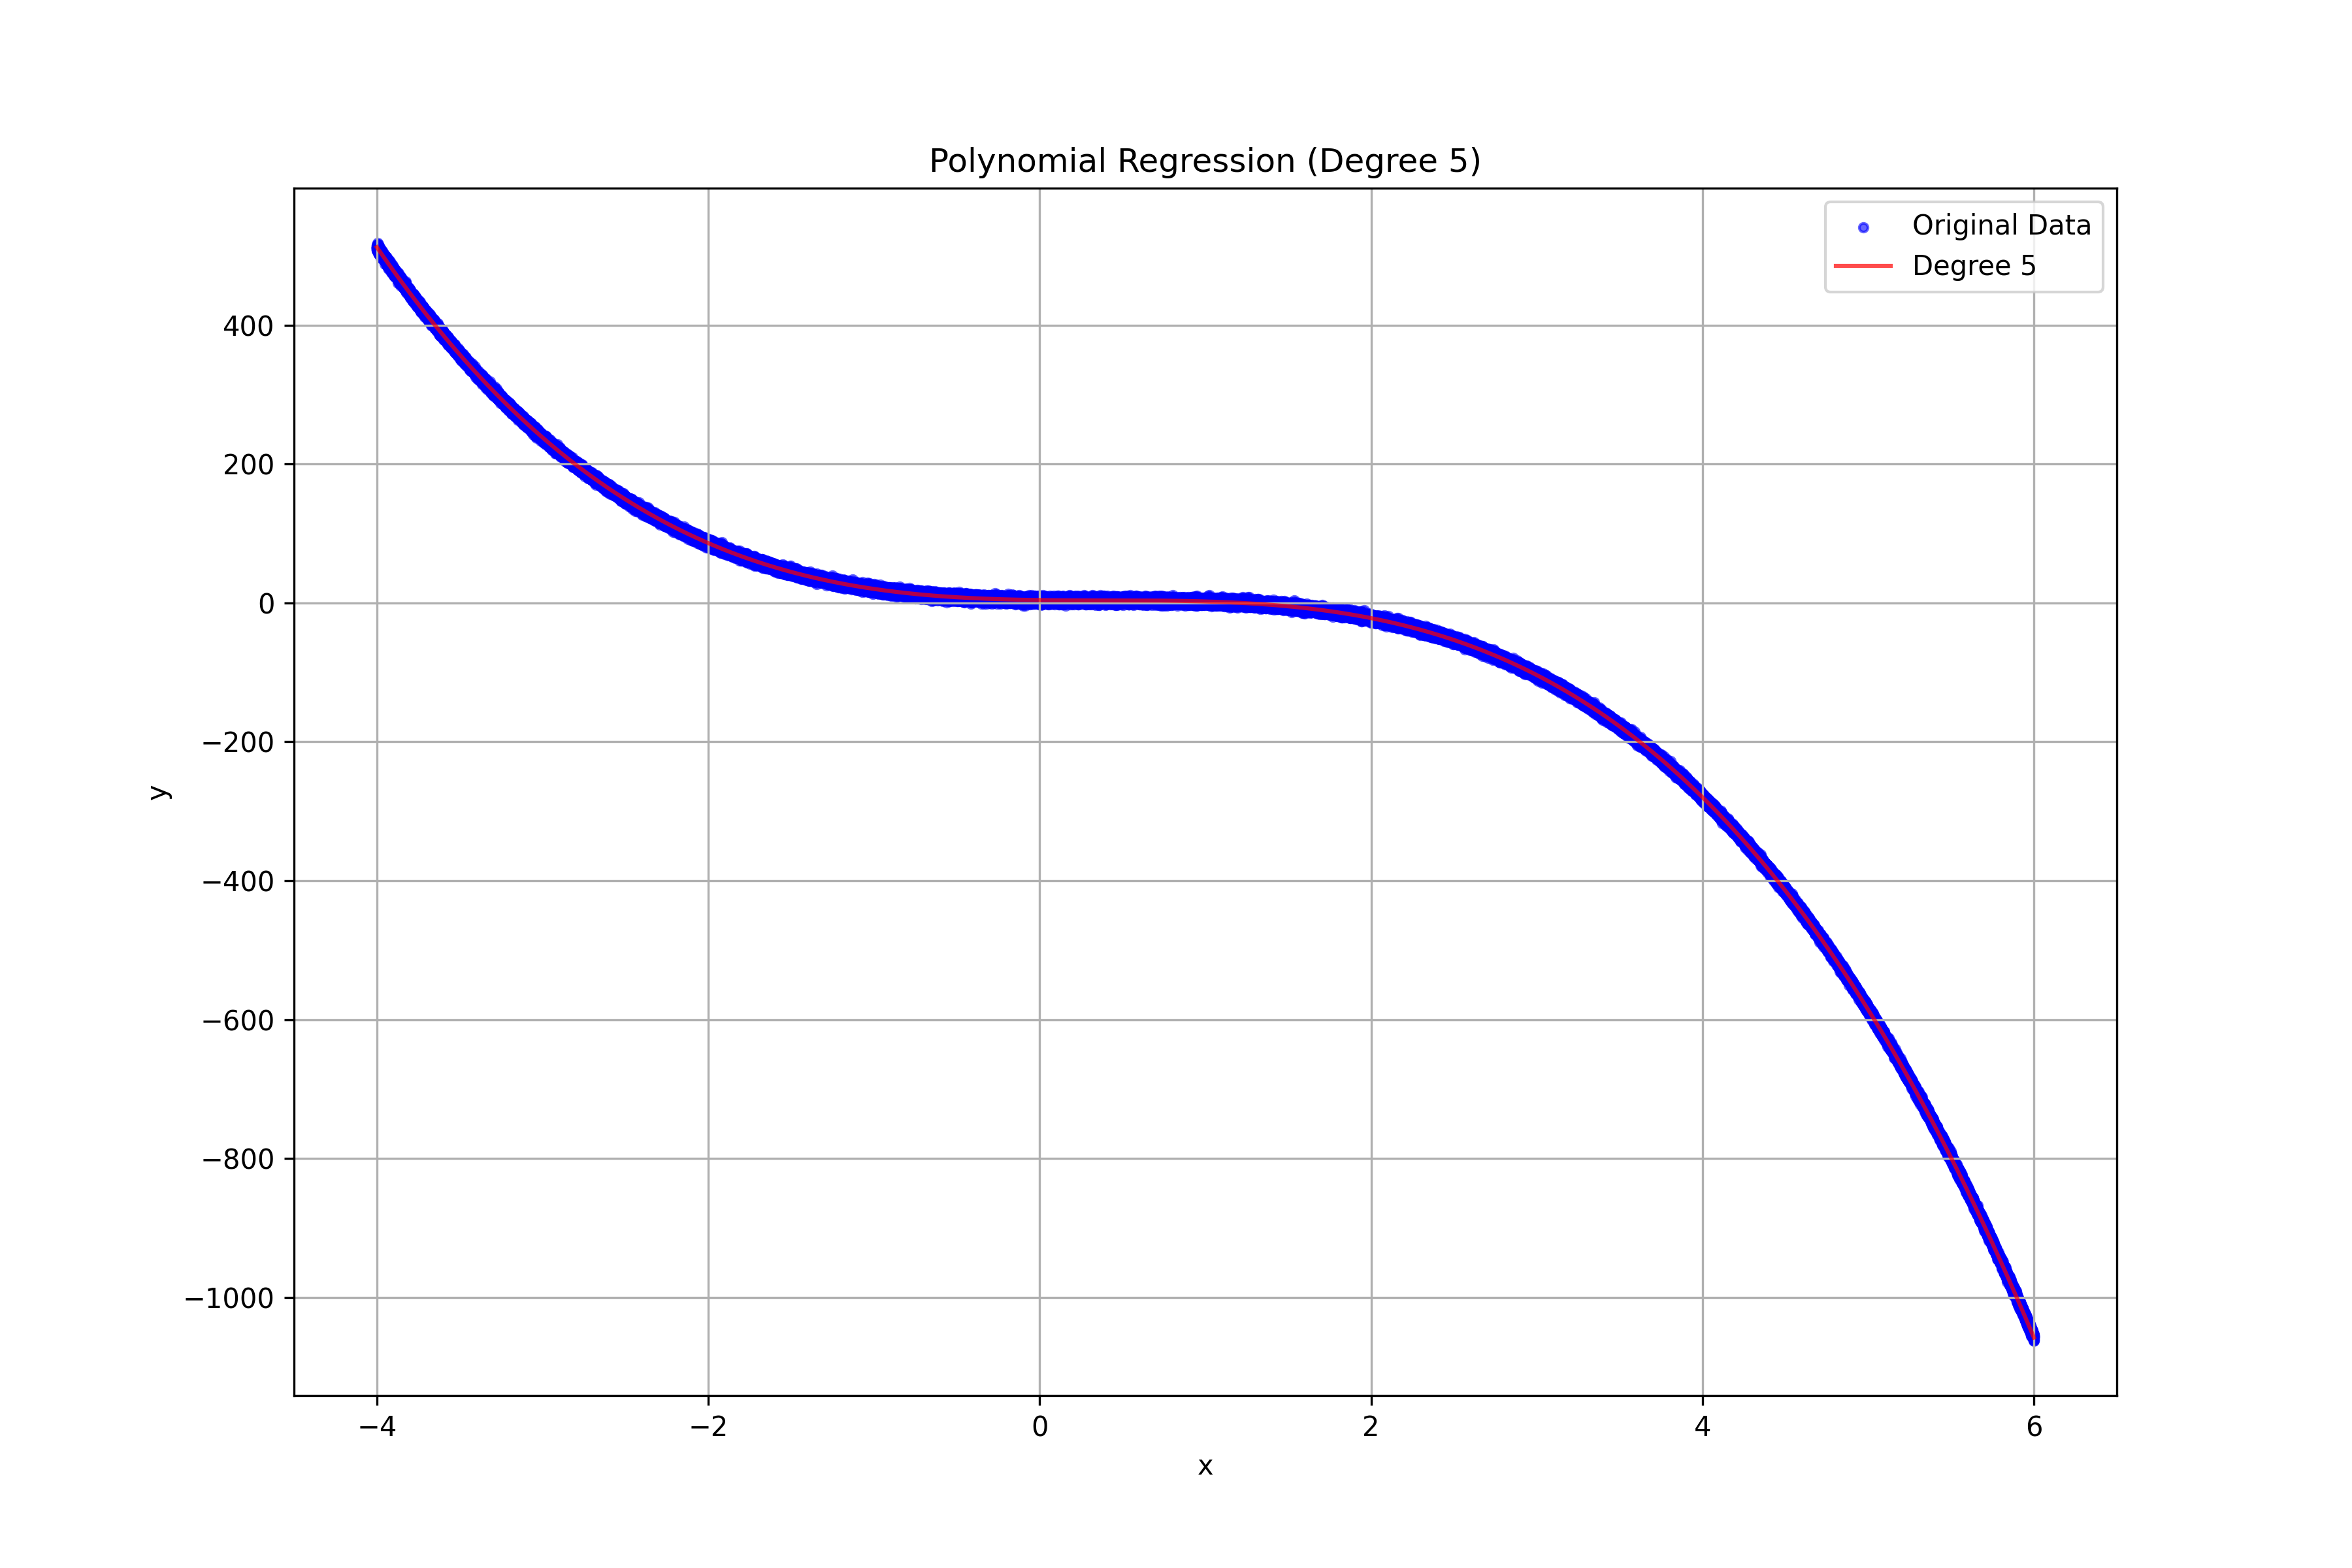
\includegraphics[width=\textwidth]{../plots/poly_reg_deg5_fold1.png}
  \centering
  \caption{Polynomial Model Degree 5}
\end{figure}

\begin{figure}[h!]
  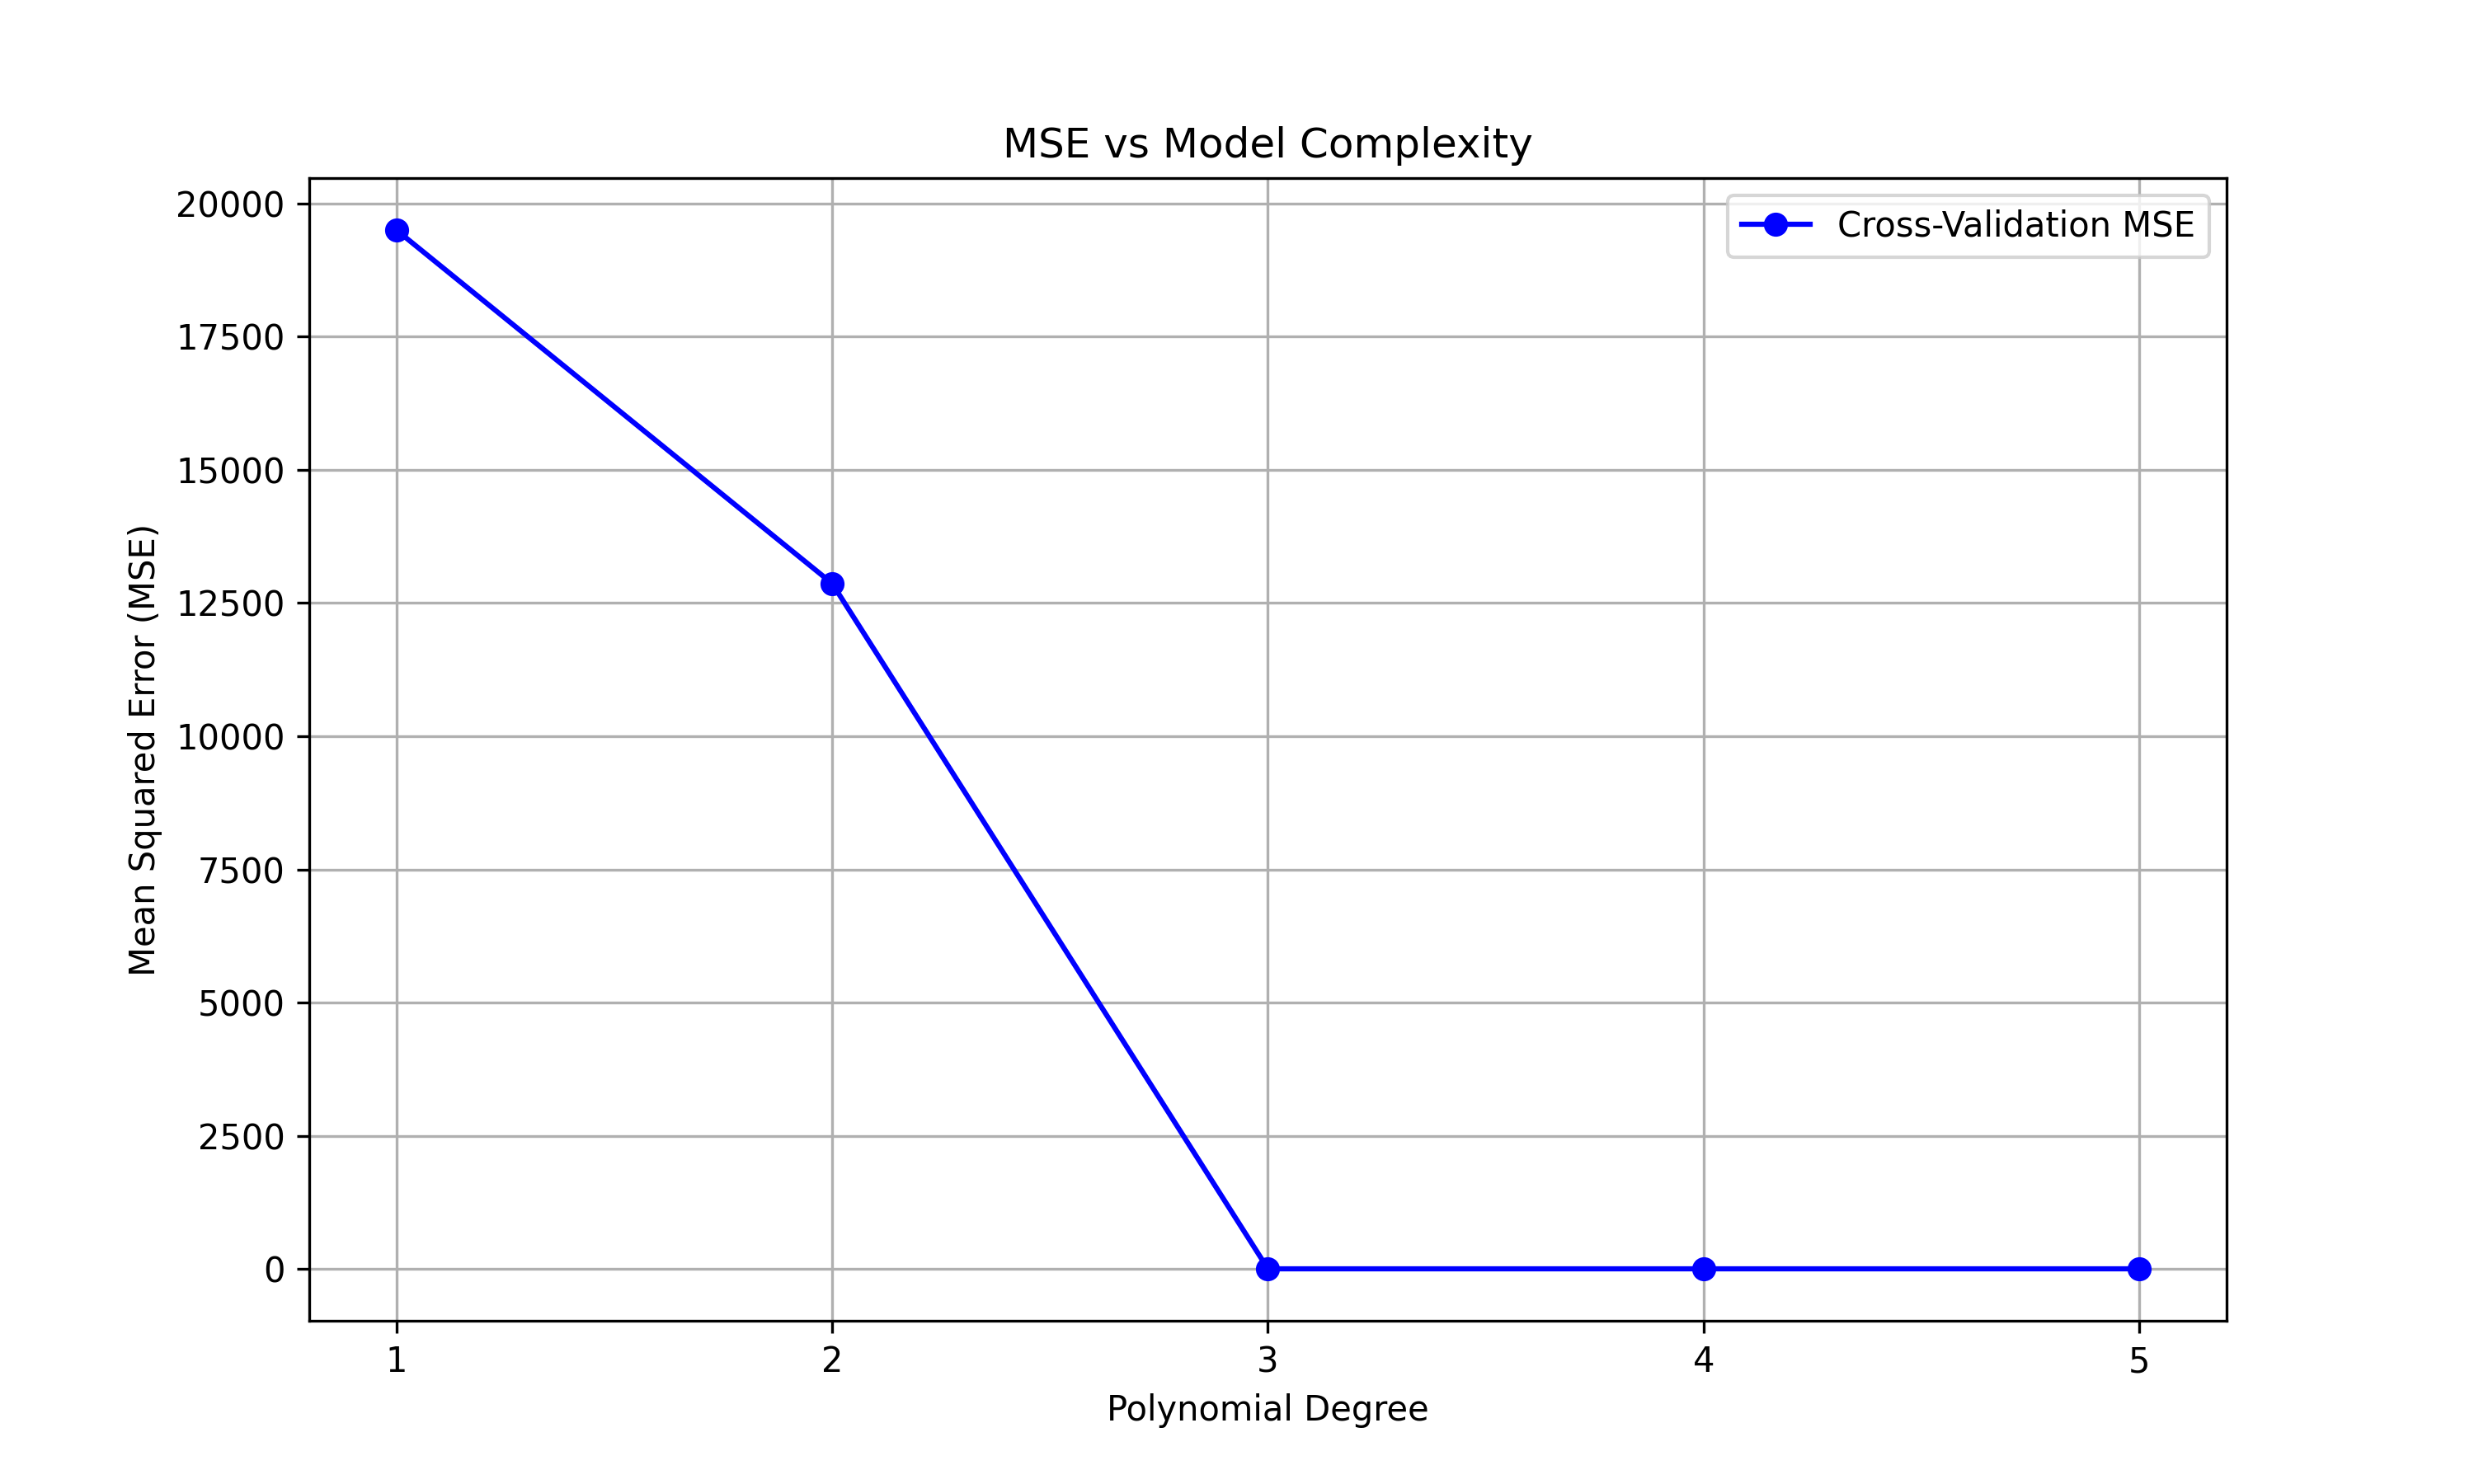
\includegraphics[width=\textwidth]{../plots/mse_vs_complexity.png}
  \centering
  \caption{MSE v. Model Complexity}
\end{figure}

\begin{figure}[h!]
  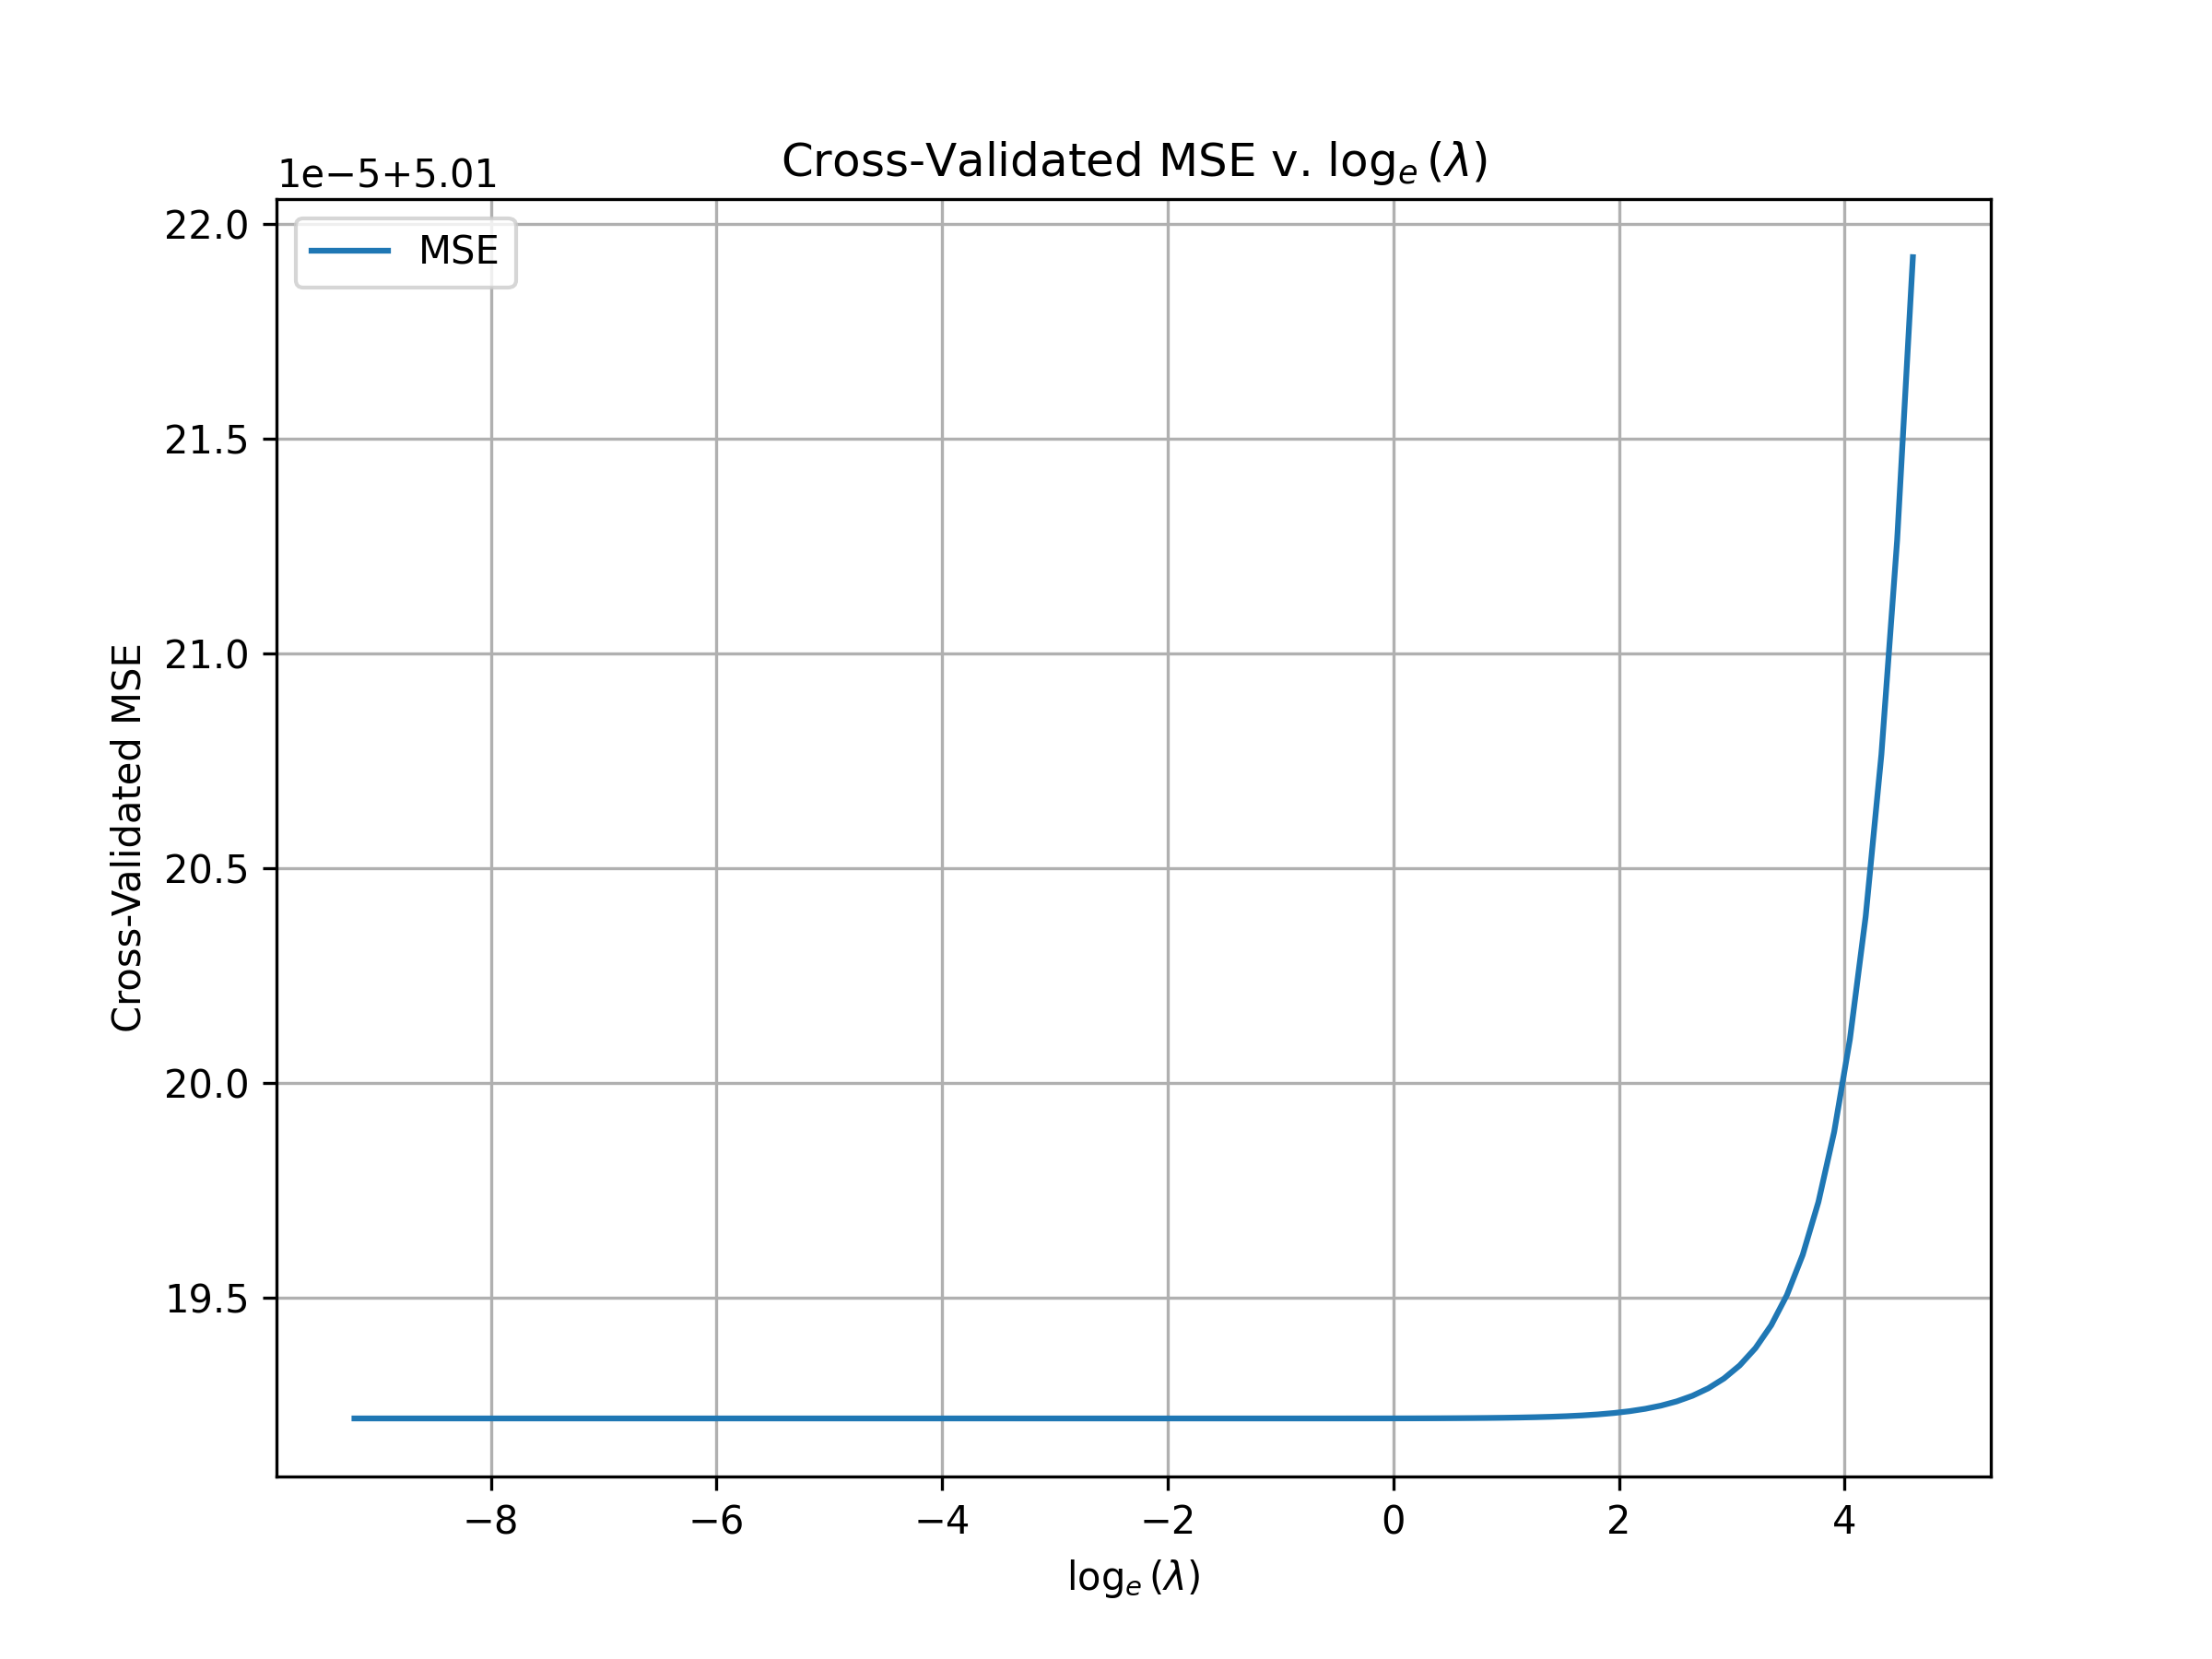
\includegraphics[width=\textwidth]{../plots/crossvalmse_vs_loglambda.png}
  \centering
  \caption{Cross-Validated MSE v. $\log_e{\lambda}$}
\end{figure}


\clearpage

\section*{Question 2}

\textbf{Solution.}
% code from q2.py
\begin{center}
  q2.py
\end{center}
\begin{lstlisting}
###########################
# Chase Lotito - SIUC F24 #
# ECE469 - Intro to ML    #
# HW2 - Question 2        #
###########################

# IMPORT LIBRARIES
import numpy as np
import pandas as pd
from sklearn.preprocessing import OrdinalEncoder    # For encoding categorical features
from sklearn.impute import SimpleImputer            # For adding missing values
from sklearn.preprocessing import StandardScaler    # For standardizing data
from sklearn.preprocessing import PolynomialFeatures
from sklearn.model_selection import cross_val_score, train_test_split, KFold
from sklearn.linear_model import LinearRegression
from sklearn.linear_model import Ridge
from sklearn.metrics import mean_squared_error
import matplotlib.pyplot as plt


# (A) DOWNLOAD HOUSING.CSV

# Get housing data
RAW_DATA = 'https://github.com/ageron/data/raw/main/housing/housing.csv'
housing = pd.read_csv(RAW_DATA)



# (B) DATA-PREPROCESSING FROM HW1

# Choose input features and output features (saved into numpy.ndarray type)
X = housing[
        ['longitude',
        'latitude',
        'housing_median_age',
        'total_rooms',
        'total_bedrooms',
        'population',
        'households',
        'median_income',
        'ocean_proximity']
    ].values
Y = housing[['median_house_value']].values

# Ocean Proximity is a categorical feature. Drop it or transform into numerical values (encode).

# Isolate the ocean_proximity data in input data X
ocean_proximity = X[:,8].reshape(-1,1)   # reshape(-1,1) to make 2D array for Ordinal
# Initalize the ordinal encoder
ordinal_encoder = OrdinalEncoder()
# Encode the ocean_proximity strings into numerical data
encoded_ocean = ordinal_encoder.fit_transform(ocean_proximity)
# Put the encoded version of ocean_proximity into input data X
X[:,8] = encoded_ocean.flatten()         # flatten to add 1D version of array back into X

# Clean the dasta by either dropping or replacing missing values

# Initialized SimpleImputer, will use the median to add missing entries
simple_imputer = SimpleImputer(strategy='median')

# Change X np ndarray into a Pandas Dataframe to use SimpleImputer
dX = pd.DataFrame(X)
dY = pd.DataFrame(Y)

# Perform SimpleImputer transformation, for both inputs X and outputs Y
imputed_data = simple_imputer.fit_transform(dX)
X = imputed_data
imputed_data = simple_imputer.fit_transform(dY)
Y = imputed_data

# Carry out feature scaling either via normalization or standardization.
std_scaler = StandardScaler()
scaled_data = std_scaler.fit_transform(X)
X = scaled_data
scaled_data = std_scaler.fit_transform(Y)
Y = scaled_data

# set test set size
test_size = 0.2

# split into testing and training set (both outputted as pd.DataFrames)
X_train, X_test, Y_train, Y_test = train_test_split(X, Y, test_size=test_size, random_state=42)




# (C) USE LINEAR REGRESSION TO DEVELOP AN ML MODEL FOR PREDICTION OF
#     'MEDIAN_HOUSE_VALUE' FOR FUTURE INPUTS AND ANALYZE TEST ERRORS
#      EXPLICITLY EXPRESS THE CORRESPONDING OPTIMAL WEIGHTS AND THE
#      FINAL LEARNED MODEL. USE GRAPHICAL REPRESENTATIONS.

# initalize and train linear model
linear_regressor = LinearRegression()
linear_regressor.fit(X_train, Y_train)   # <-- train model here

# extract the optimal weights from the ML model
weights = linear_regressor.coef_.flatten()      # flatten makes it a normal list

# test model 
Y_train_predicted = linear_regressor.predict(X_train)
Y_test_predicted = linear_regressor.predict(X_test)

# calculate mean square error
mse_train = mean_squared_error(Y_train, Y_train_predicted)
mse_test = mean_squared_error(Y_test, Y_test_predicted)

# VISUALIZATION
# print out results of linear model
print("--------------------")
print("LINEAR MODEL RESULTS")
print("--------------------")
print(f"Model Weights: {weights}")
print(f"MSE (train): {mse_train*100:.2f}%")
print(f"MSE (test): {mse_test*100:.2f}%")

# Plot predicted vs actual values
plt.scatter(Y_test, Y_test_predicted, marker='o', s=0.75, c='#32a852', alpha=0.95, label='Pred v. Actual')     # plot predicted against actual, if diagonalized, well fit.
plt.plot([min(Y_test), max(Y_test)], [min(Y_test), max(Y_test)], label='Ideal Model',color='red', linewidth=2)
plt.xlabel("Actual Median House Value")
plt.ylabel("Predicted Median House Value")
plt.title("Predicted Median House Value vs Actual Median House Value")
plt.legend()
plt.savefig("plots\\q2_pred_vs_actual.png", dpi=300)
plt.close()

# Plot the Learned Weights
# Coefficients of the model
#feature_names = ['longitude', 'latitude', 'housing_median_age', 'total_rooms', 
#                 'total_bedrooms', 'population', 'households', 'median_income', 'ocean_proximity']
#
#plt.barh(feature_names, weights)
#plt.xlabel("Model Weights $w_i$")
#plt.title("Linear Regression Feature Weights")
#plt.show()
#plt.close()



# (D) USE CROSS-VALIDATION TECHNIQUES TO IMPROVE THE GENERALIZATION OF THE MODEL AND ANALYZE
#     THE ROOT MEAN SQUARE ERROR (RMSE). USE GRAPHICAL ILLUSTRATIONS.

# parameters
lambdas = np.logspace(-4, 2, 100)  # lambdas for ridge
kf = KFold(n_splits=10, shuffle=True, random_state=1)

# store cross-validation results
mse_values = []

# perform cross-validation for each lambda
for alpha in lambdas:
    ridge = Ridge(alpha=alpha)

    # calc mse using cross_val_score
    mse = -cross_val_score(ridge, X, Y, cv=kf, scoring='neg_mean_squared_error').mean()
    mse_values.append(mse)

# find lambda with best minimum mse
best_lambda = lambdas[np.argmin(mse_values)]
print("--------------------")
print("RIDGE REGULARIZATION")
print("--------------------")
print(f"Best lambda (w/ minimum MSE): {best_lambda:.2f}")
print(f"Minimum MSE: {np.min(mse_values)*100:.2f}%")

# fit model with best lambda
ridge_best = Ridge(alpha=best_lambda)
ridge_best.fit(X_train, Y_train)

# testing x values
Y_test_ridge_pred = ridge_best.predict(X_test)

# plot rmse vs. ln(lambda)
plt.figure(figsize=(8,6))
plt.plot(np.log(lambdas), np.sqrt(mse_values), c="#570710",label='MSE')
plt.xlabel('$\\log_e (\\lambda)$')
plt.ylabel('Cross-Validated RMSE')
plt.title('Q2: Cross-Validated RMSE v. $\\log_e (\\lambda)$')
plt.grid(True)
plt.legend()
plt.savefig('plots\\q2_crossvalmse_vs_loglambda.png', dpi=300)
plt.close()
\end{lstlisting}

\bigskip
We can plot, like in Figure \ref{fig:predvact}, the predicted values against the actual values to see how well the learned model works. If the predicted values (green) lie along the same line as the actual values (red), then the model is ideal. However, we see the linear model has a large spread, which means the model is most likely not complex enough to model the input features.


\begin{figure}[h!]
  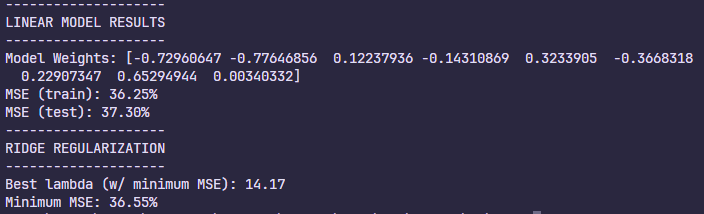
\includegraphics[width=0.75\textwidth]{../outputs/q2.png}
  \centering
  \caption{q2.py Terminal Output}
  \label{fig:q2out}
\end{figure}

From Figure \ref{fig:q2out}, we can write the equation for the final learned model:

\begin{align*}
  y(\vb{x}) = -0.7296x_1 + -0.7765x_2 + 0.1224x_3 &+ -0.1431x_4 + 0.3234x_5 \\
  &+ -0.3668x_6 + 0.2291x_7 + 0.6529x_8 + 0.0034x_9 
\end{align*}

Where the input vector \(\vb{x}\) is defined as:

\begin{equation*}
  \vb{x} = \begin{bmatrix}
    x_1:  &\text{longitude} \\
    x_2: &\text{latitude} \\
    x_3: &\text{housing median age} \\
    x_4: &\text{total rooms} \\
    x_5: &\text{total bedrooms} \\
    x_6: &\text{population} \\
    x_7: &\text{households} \\
    x_8: &\text{median income} \\
    x_9: &\text{ocean proximity} \\
  \end{bmatrix}
\end{equation*}

\begin{figure}[h!]
  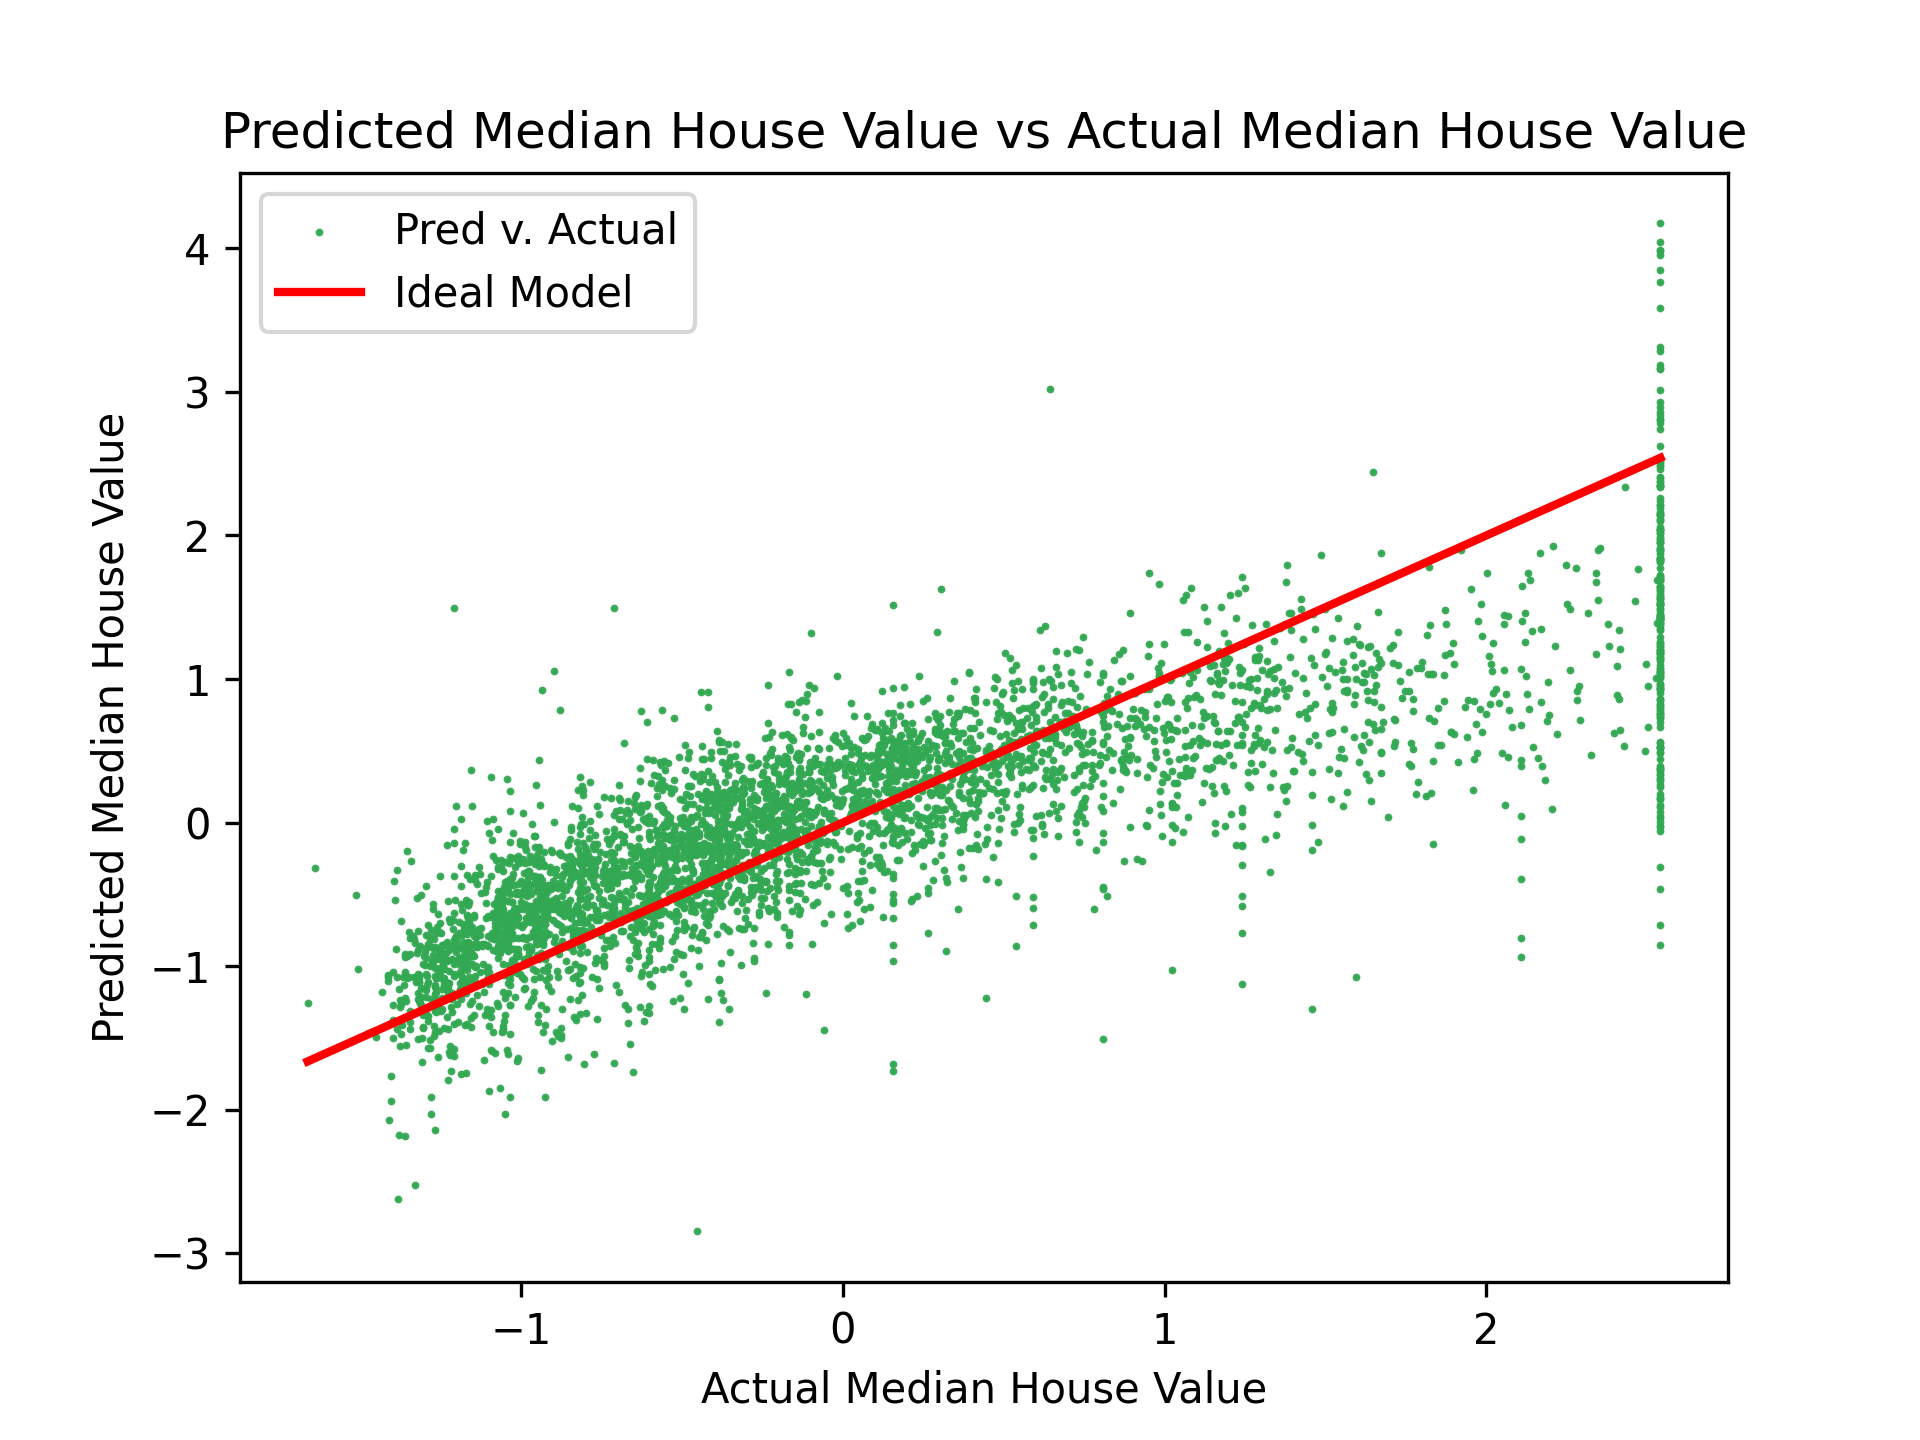
\includegraphics[width=\textwidth]{../plots/q2_pred_vs_actual.png}
  \centering
  \caption{Predicted Median House Value v. Actual Median House Value}
  \label{fig:predvact}
\end{figure}

\begin{figure}[h!]
  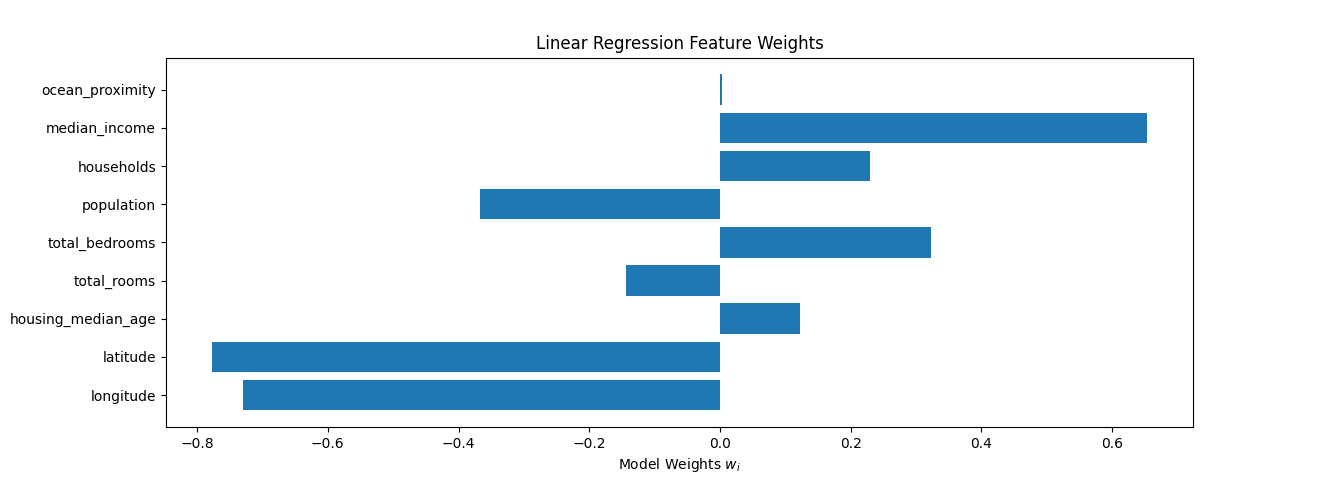
\includegraphics[width=\textwidth]{../plots/q2_model_weights.png}
  \centering
  \caption{Model Weights}
  \label{fig:weights}
\end{figure}


\begin{figure}[h!]
  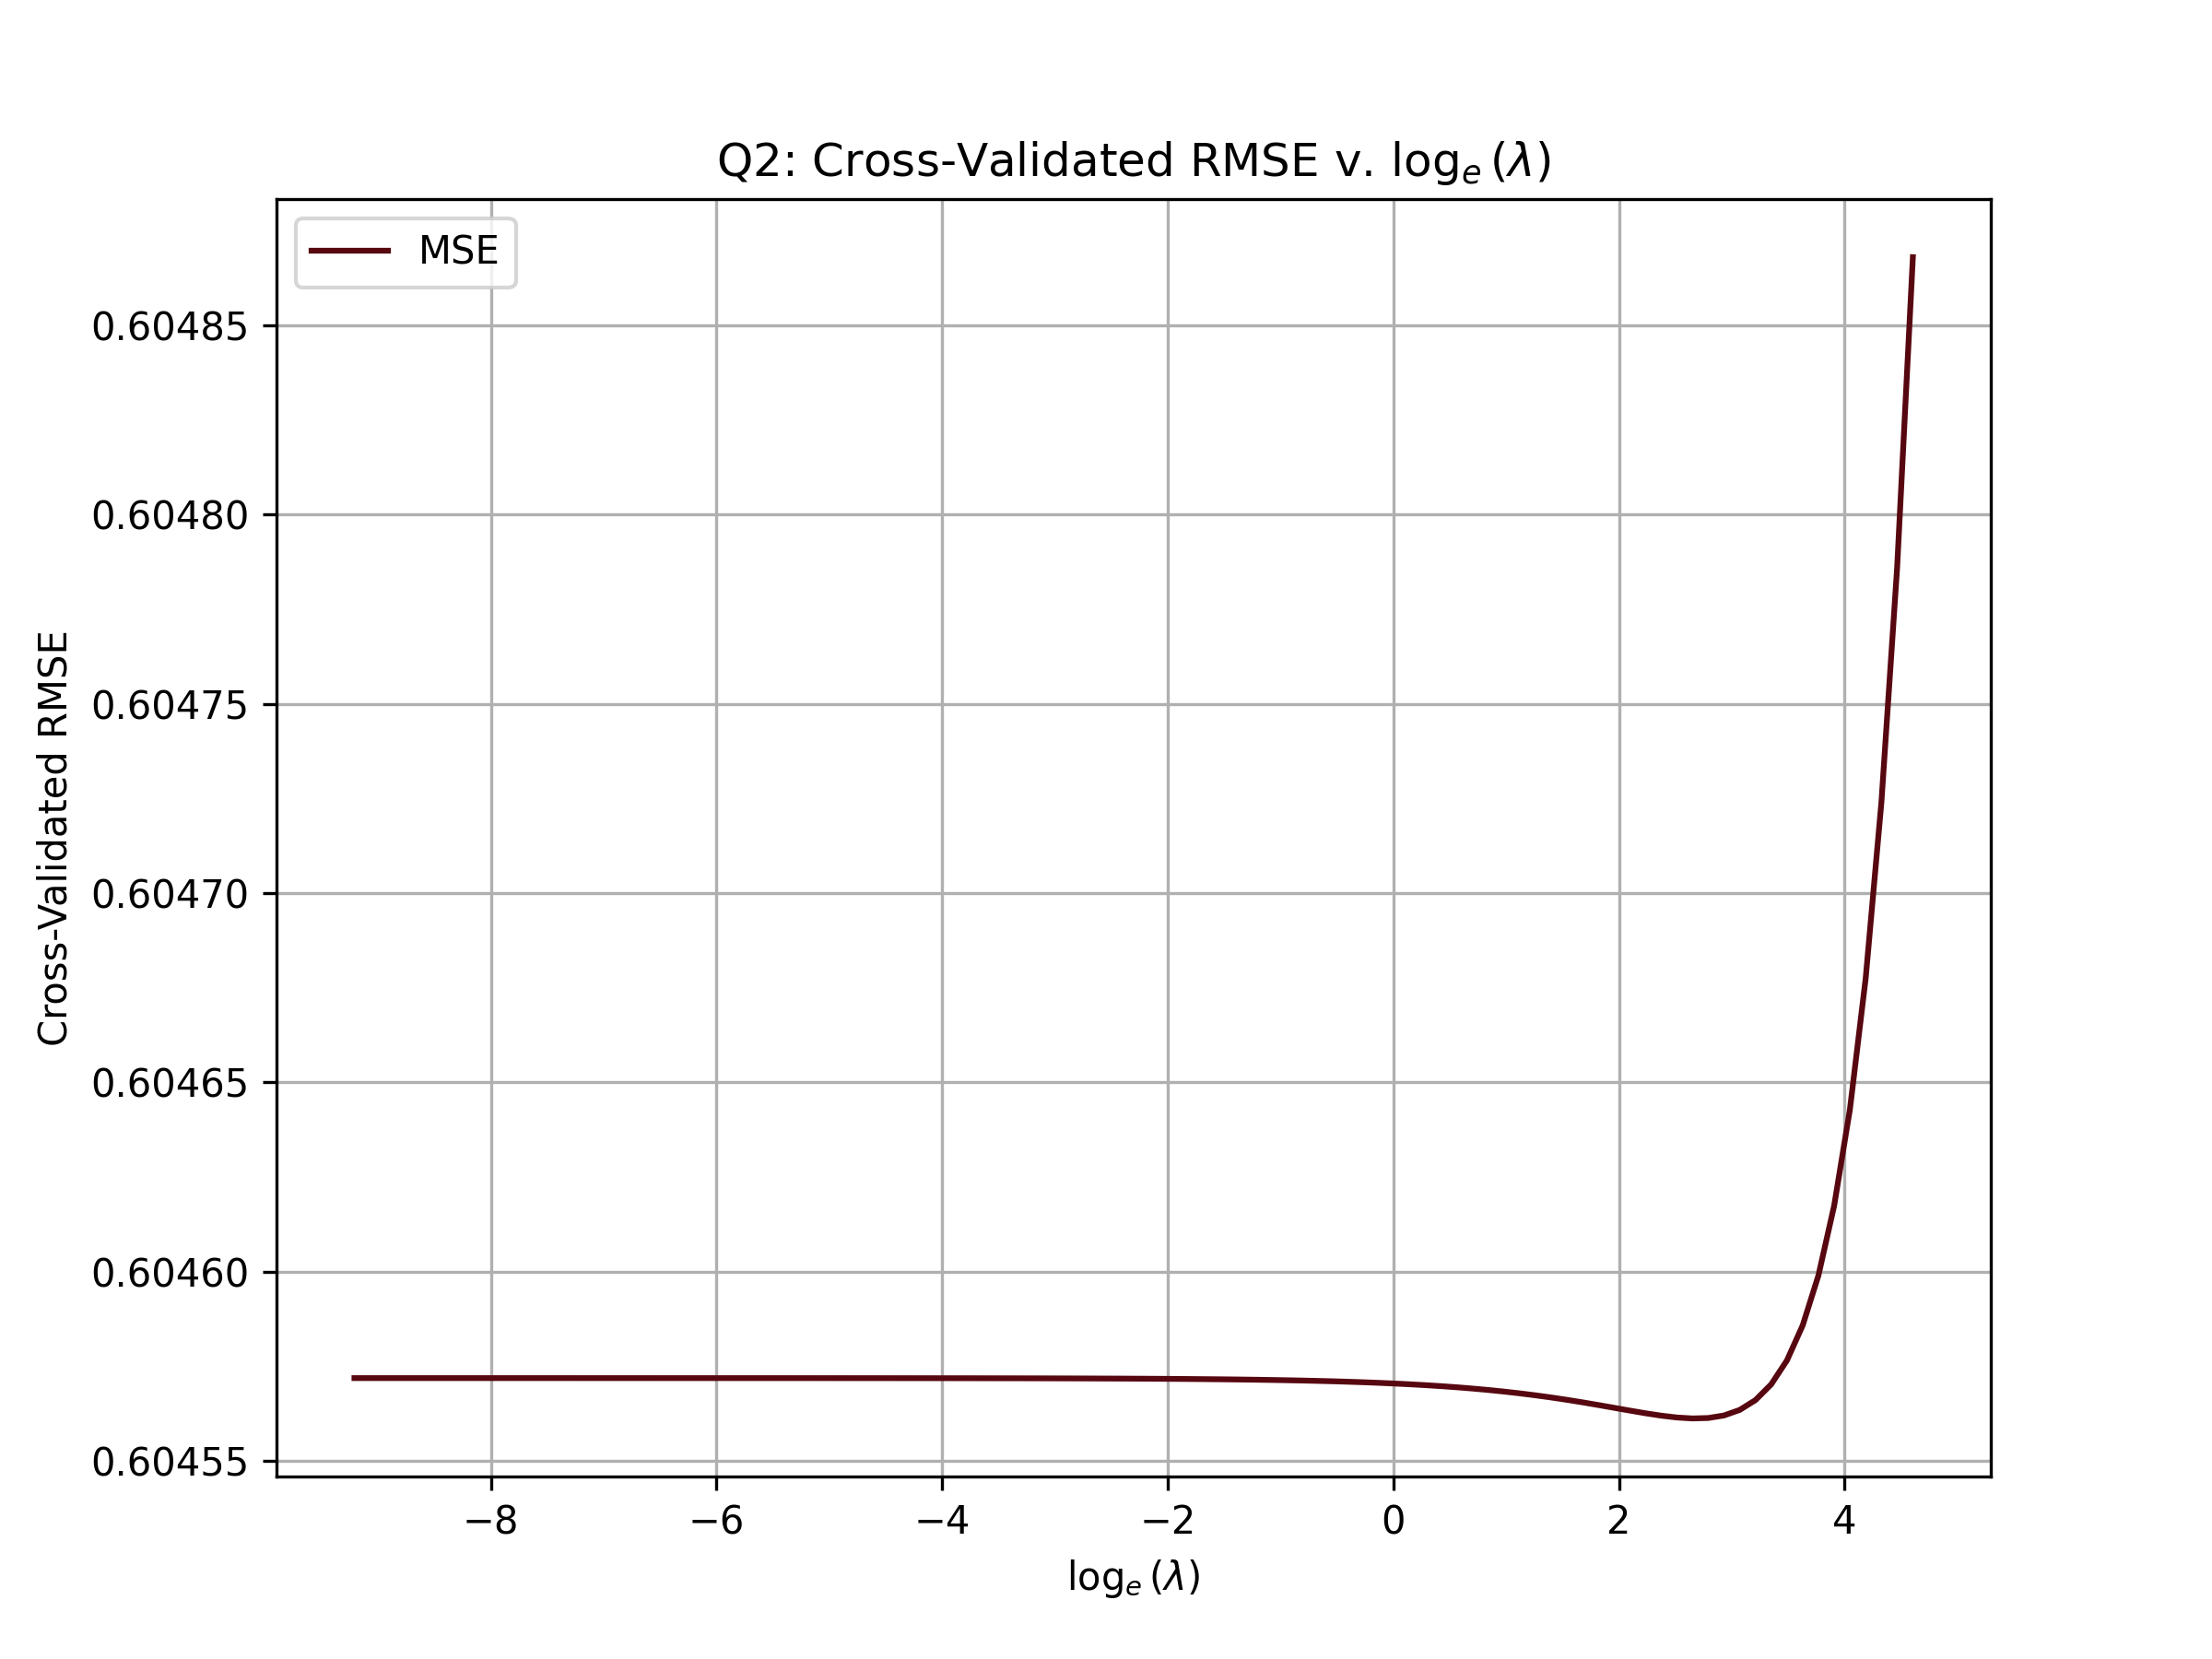
\includegraphics[width=\textwidth]{../plots/q2_crossvalmse_vs_loglambda.png}
  \centering
  \caption{Cross-Validated RMSE v. \(\log_e{\lambda}\)}
\end{figure}






\end{document}